\makeatletter
%\newcommand{\rmnum}[1]{\romannumeral #1 }
%\newcommand{\Rmnum}[1]{\expandafter\@slowromancap\romannumeral #1@}
\makeatother
\ifpdf
\graphicspath{{Chapter2/Chapter2Figs/PNG/}{Chapter2/Chapter2Figs/PDF/}{Chapter2/Chapter2Figs/}}
\else
\graphicspath{{Chapter2/Chapter2Figs/EPS/}{Chapter2/Chapter2Figs/}}
\fi

\chapter{Cache Side-Channel Attacks}
	\label{chapter_sca}

	Timing Side-Channel Attacks (SCAs) rely on measuring cache misses through memory access latency. We hypothesise that cache self-invalidation reduces observable timing variations, thus masking the leakage of side-channel information. In general, SCAs are a method of gathering information through physical observations of a system. The attack does not seek weaknesses in software algorithms (usually cryptographic), instead it relies on the physical properties of the system. Common attacks include: timing analysis, power monitoring, electromagnetic emanations, and many more. 
	
	In this chapter I focus on timing memory operations and extracting useful information correlated with the behaviour of a critical application, the Victim. If the Victim application is a cryptosystem then the analysis of its memory usage may compromise security. AES is a widely used cryptographic algorithm and it is often used as a target in SCA research. Timing attacks on AES have shown successful cryptographic key extraction through cache side-channels \cite{Brumley03,Percival05,Bonneau06_0}. 
	In AES, the key value and the plain text affect the memory usage of the algorithm. Profiling the memory usage will allow an estimation of the key with a high degree of certainty. 
	
	Extraction of security critical information through side-channels is well understood; I will focus primarily on reducing cache side-channel leakage rather than key extraction or data decryption.

\section{Effects of Coherence on SCAs}
	Coherence mechanisms such as snooping or directories are designed to provide shared memory communication. These schemes focus on efficient shared memory updates and do not actively conceal any memory latency variations. Compared to a single processor system, a multiprocessor should provide no additional SCA protection other than misdirection through parallel software execution. SCAs work best when the attacking code and the Victim code are collocated (operating on the same processing element or memory segment). Successful attacks are possible even when the applications are not collocated, information can be extracted by timing shared or main memory accesses \cite{Ristenpart09,Brumley11,Hund13,Yarom14}.
	
	I have established the behaviour of time-based coherence in previous chapters. The scheme  ejects cached data at regular intervals, thus, adding timing entropy and masking some of the cache side-channel leakage. This system property is inherent and does not require any additional support. SCA mitigation can be further improved by making some minor software modifications.

\section{SCAs on BERI/CHERI}
	\textcolor{red}{The CHERI architecture is designed to provide fine grained memory protection. Capabilities allow fixed memory segment allocation for each application. Allocated memory segment are exclusive to each process. This mechanism provides robust protection against software attacks such as buffer overflows. However, the capability model does not protect against SCAs.}

	\textcolor{red}{Capabilities provide memory bounds for application data. This data is stored in memory just like any other data. Capabilities enforce memory address bounds, but they do not directly affect cached data. Capabilities themselves are stored in memory but tagged with an additional bit to differentiate them from non-capability data.}

	\textcolor{red}{Cache SCAs attempt to determine the memory usage of a particular application and thereby uncover the operations performed. As far as a spy program is concerned, the memory data usage of a capability-protected application and a traditionally compiled application is similar. Major differences will be linked to capability memory operations and any additional memory required for storing capabilities. Capabilities do not replace paging, so any SCAs designed to exploit TLB paging will remain effective. If a cryptographic algorithm is executed on a capability system, it will be safe against memory leaks but not against SCAs.}

	\subsection{Cryptography and SCAs}
		The behaviour of a cryptographic algorithm is dependant on the input data, key, or often both. A variation in any one of the parameters will usually result in different cryptographic steps. Encryption algorithms such as RSA, ElGamal, and Digital Signature Algorithm use modular exponentiation in one of the steps \cite{Daly02}. This operation calculates the remainder (z) when as integer (x) is raised to the power (p) and divided by a positive integer (y). This algorithm is iterative and the input parameters will affect memory usage. The memory usage can diverge to the extent that keys can be delivered from coarse side-channel memory behaviour observations.
	
	\subsection{State of the art SCA Mitigation}
		A number of SCA mitigation techniques have already been mentioned in Chapter \ref{chapter_background}. They can be broadly grouped into four categories: 
		
		\begin{enumerate}
			\item OS-driven mitigation techniques such as removal of caching privileges, cache flushing, and skewing timing device measurements.
			\item Algorithm specific masking modifies the behaviour of a cryptographic algorithm. In case of AES, the memory footprint of each encryption round can be kept constant. Loading the entire s-box into the cache would ensure uniform access.
			\item Dedicated hardware modules for popular cryptographic schemes can be added to commercial systems. These dedicated accelerators bypass the caches altogether.
			\item Modified cache behaviour can improve the level of side-channel masking. Techniques such as cache partitioning, pseudo-random or random cache misses, and non-deterministic prefetching.
		\end{enumerate}
	
	\subsection{Exploiting Time-Based Coherence for SCA Mitigation}
		Traditional cache coherence mechanisms are designed for parallel performance and memory consistency. The addition of a coherence scheme affects memory behaviour by adding a level of indirection.
		
		The time-based cache coherence mechanism is simple to implement in the context of BERI architecture. A side-effect of self-invalidating private caches is a subtle masking of an applications memory footprint. The level of mitigation provided for collocated Attacker-Victim applications may be equivalent to the applications running on completely independent cores.
		
		The coherence model is not very effective at mitigating attacks aimed at lower levels of memory, such as the shared cache or main memory. However, aggressive self-invalidation adds noise to time measurements when attacking the lower levels. This uncertainty can be overcome through higher SCA sampling. 
	
\section{BERI SCA Analysis}
	Modern processor designs incorporate multi-tired caches with a diverse behaviour, making side-channel attacks much more difficult, as demonstrated by Mowery et al. \cite{Mowery12}. The BERI memory subsystem is fairly simple compared to commercial designs. Direct mapped caches, in-order execution, no write buffers, no memory access reordering, simple prefetching, and other factors make BERI highly susceptible to SCAs. The BERI platform is ideal for SCA mitigation analysis as the memory architecture does not mask side-channels. Direct mapped caches ensure interference between the Victim and Trojan (attacker) data, this interference is less certain in set-associative caches. In-order execution and no memory reordering ensures a sequential attack.

	\subsection{Memory Footprint Analysis}
		Information leakage of a memory system is best quantified through a controlled experiment that does not rely on cryptographic algorithms. Attacks usually described in SCA research focus on cryptographic properties that may not be applicable to other programs. AES attacks include: One-Round, Two-Round, Evict+Time, Prime+Probe, and others \cite{Osvik06}. 
		
		The first two attacks are directly aimed at AES, whereas the other two can be applied to general applications. The Prime+Probe attack is one of the stronger options. An attacker plants some Trojan code in the desired system. The objective is to interfere with cache behaviour and thereby extract useful side-channel information. This style of attack has been tested on both directory and time-based coherence protocols; in simulation with no OS and on FPGA whilst running FreeBSD.
		
		The Prime+Probe attack can be applied on a varying scale, from a single memory location to an entire cache. Coarse grained timing measurements and a generally noisy system might force the attacker to use a single cache line attack. Figure \ref{prime_and_probe} shows an example of a Prime+Probe attack. In order to simplify the explanation, let us assume that the cache only holds 4 lines and the Victim application requires only 1 cache line for its data. The SCA steps are listed below:
		
		\begin{figure}[!h]
		\centering 
			\makebox{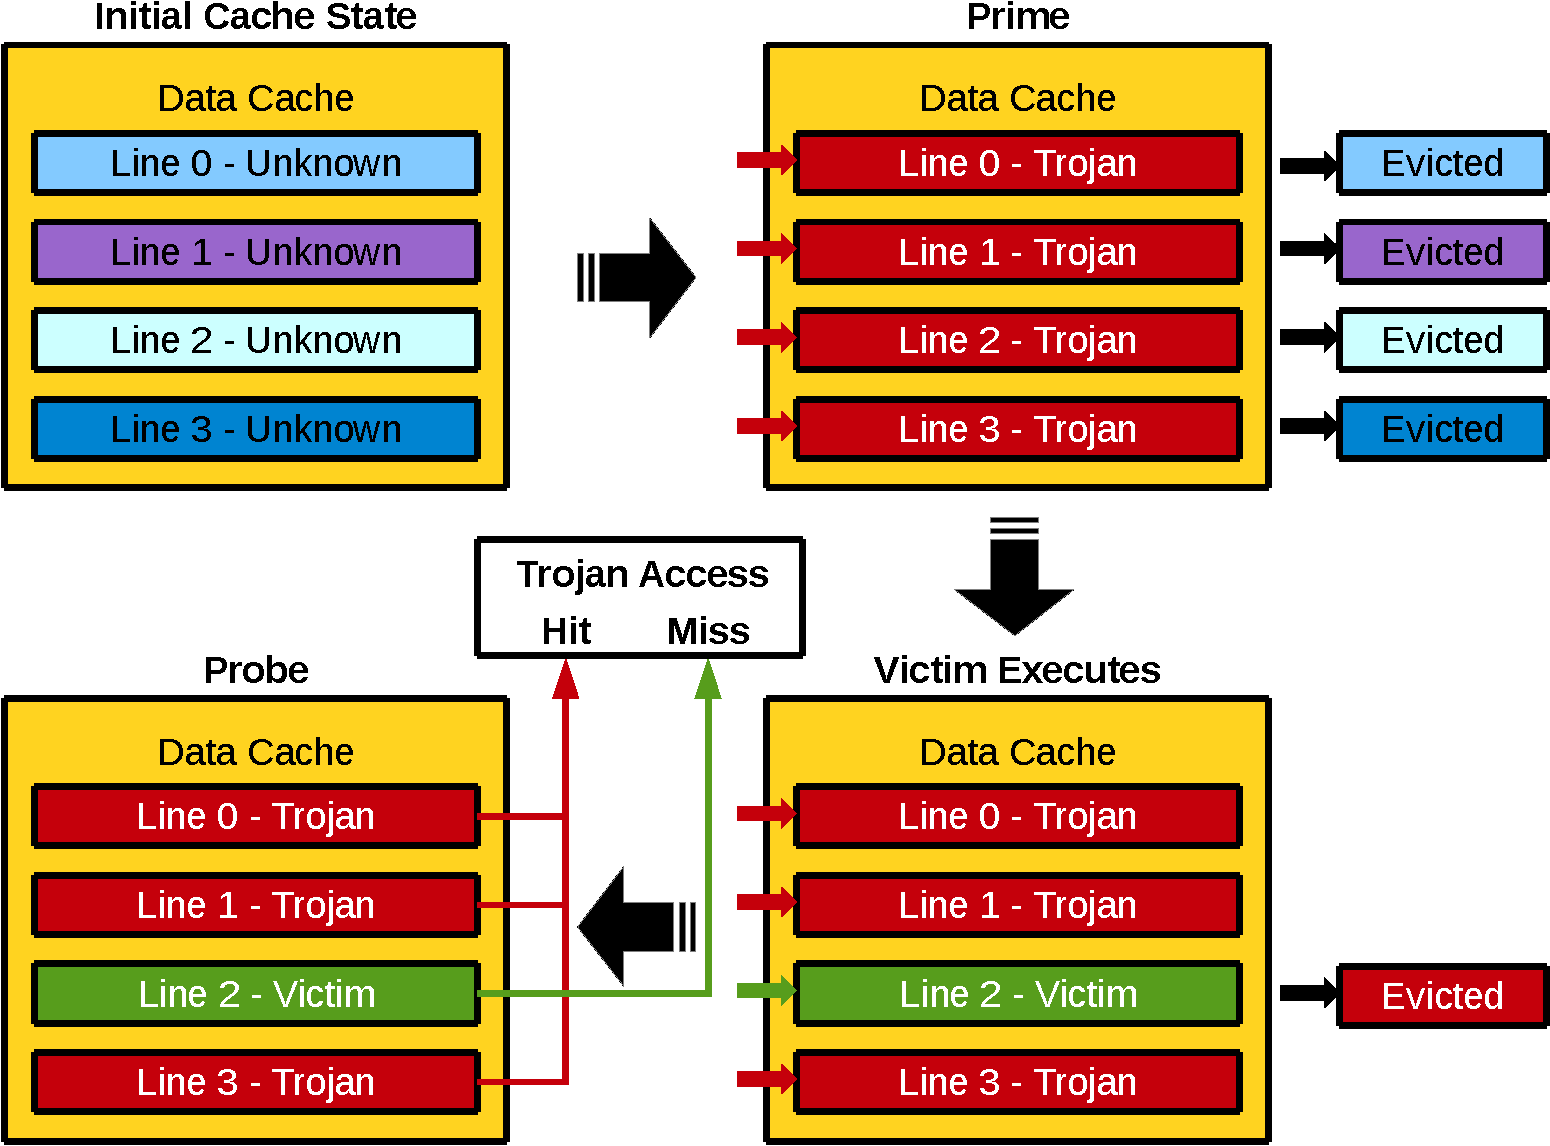
\includegraphics[width=\textwidth,height=\textheight,keepaspectratio]{prime_and_probe}}
			\caption{Prime+Probe attack} 
			\label{prime_and_probe}
		\end{figure}
		%\vspace{-5mm}
		
		\begin{enumerate}
			\item Initial Cache State: At this point the cache is in an unknown state, likely holding unrelated or invalid data.
			\item Prime: The Trojan begins by loading its own data into every line of this cache (4 memory lines in this example).
			\item Victim Executes: The Victim application is allowed to execute. In this example the application uses line 2 of the cache to hold its data. Thus, data previously held in line 2 is evicted (Trojans data).
			\item Probe: The Trojan measures memory latency by reading back its own data from memory, any misses in the cache will add latency, hardware time counters or OS counters can be used. Since line 2 has been evicted, the Trojan will be able to determine that an application executed prior to the Probe phase accessed line 2.
		\end{enumerate}
		
		The example shown is very simple but when it is scaled up to a full system, the Trojan will be able to determine the memory footprint of the Victim application. In the case of AES, this would allow an attacker to recursively work out the cryptographic key used for a certain piece of data. The same attack principle can be applied to a variety of applications, but most mitigation techniques only focus on cryptographic algorithms.

	\subsection{Effects of Coherence on SCAs}
		Multi-threaded applications can benefit from some masking effects produced by cache coherence. Any invalidations or updates through a coherence network can cause cache performance variations, making accurate side-channel measurements more challenging. If the Trojan application is run synchronously with the Victim, the programs may not be collocated. Thus, to observe Victim behaviour the Trojan requests will need to access shared memory. In this discussion I will mostly focus on single threaded applications in order to simplify the analysis. 
		
		\subsubsection{Directory Coherence -- SCA}
			This coherence protocol is designed to efficiently cache most frequently used data, update stale memory lines, and eliminate false sharing. The Prime+Probe attack relies on evictions caused by the cache usage of a critical application with the Probe phase revealing the memory usage.
			
			%\textcolor{red}{I have found that under appropriate OS testing conditions a multiprocessor system might be more vulnerable to SCAs, compared to a uniprocessor. The OS exploits the multi-threaded nature of the multiprocessor architectures to distribute workloads and achieve higher efficiency. Thus, other cores can As a result, the probe measurements contain less noise; generated by other processes, interrupts, exceptions, etc. These results are further illustrated in Section \ref{os_prime_probe_attack}.}
			
			The complex memory architecture of a multiprocessor systems often adds a layer of SCA indirection. However, multi-threading may still benefit an attacker. When the Trojan and Victim applications are executed on the same CPU, remaining cores can handle the OS and other processes. A uniprocessor system may add more noise to the Trojan timing results, due to interference from other processes. I have tested SCAs in a very controlled environment which showed more consistent results on the directory-based system. These results are further illustrated in Section \ref{os_prime_probe_attack}.
		
		\subsubsection{Time-Based Coherence -- SCA}	
			This coherence protocol adds unpredictability to cache behaviour by default. The protocol evicts data based on a set lifespan, clearing any stale data. Increasing the miss rate of a cache is not usually desirable, but when dealing with side channels, memory entropy could be beneficial.
			
			The Prime+Probe attack relies on controlled cache data eviction; random memory purging will not yield desired timing information. This is precisely what a time-based coherent system is able to achieve. When the attacker loads data into the cache during the Prime phase, each memory line is assigned a maximum lifespan. When this value is exceeded, the line is evicted. If sufficient time passes between the Prime and Probe phases, the Probe stage will observe data misses and no hits in the private cache. Thus, the coherence mechanism is introducing some SCA mitigation. The coherence mechanism will also have a low performance impact on the critical application (depends on the selected time-out).
			
			Another beneficial trick in favour of time-based coherence is the behaviour of SYNC instructions. As previously mentioned in Section \ref{sync_behaviour}, these instructions ensure that all memory operations prior to SYNC have completed, and all data has been marked invalid. The later is an excellent SCA mitigation mechanism since it acts as a single instruction flush. If a SYNC is used before or preferably after the critical application, it ensures that any Trojan data that might be in the cache is evicted. Importantly, SYNC will also evict all data belonging to the critical application (Figure \ref{prime_and_probe_time_based}). 
			
			\begin{figure}[t]
			\centering 
				\makebox{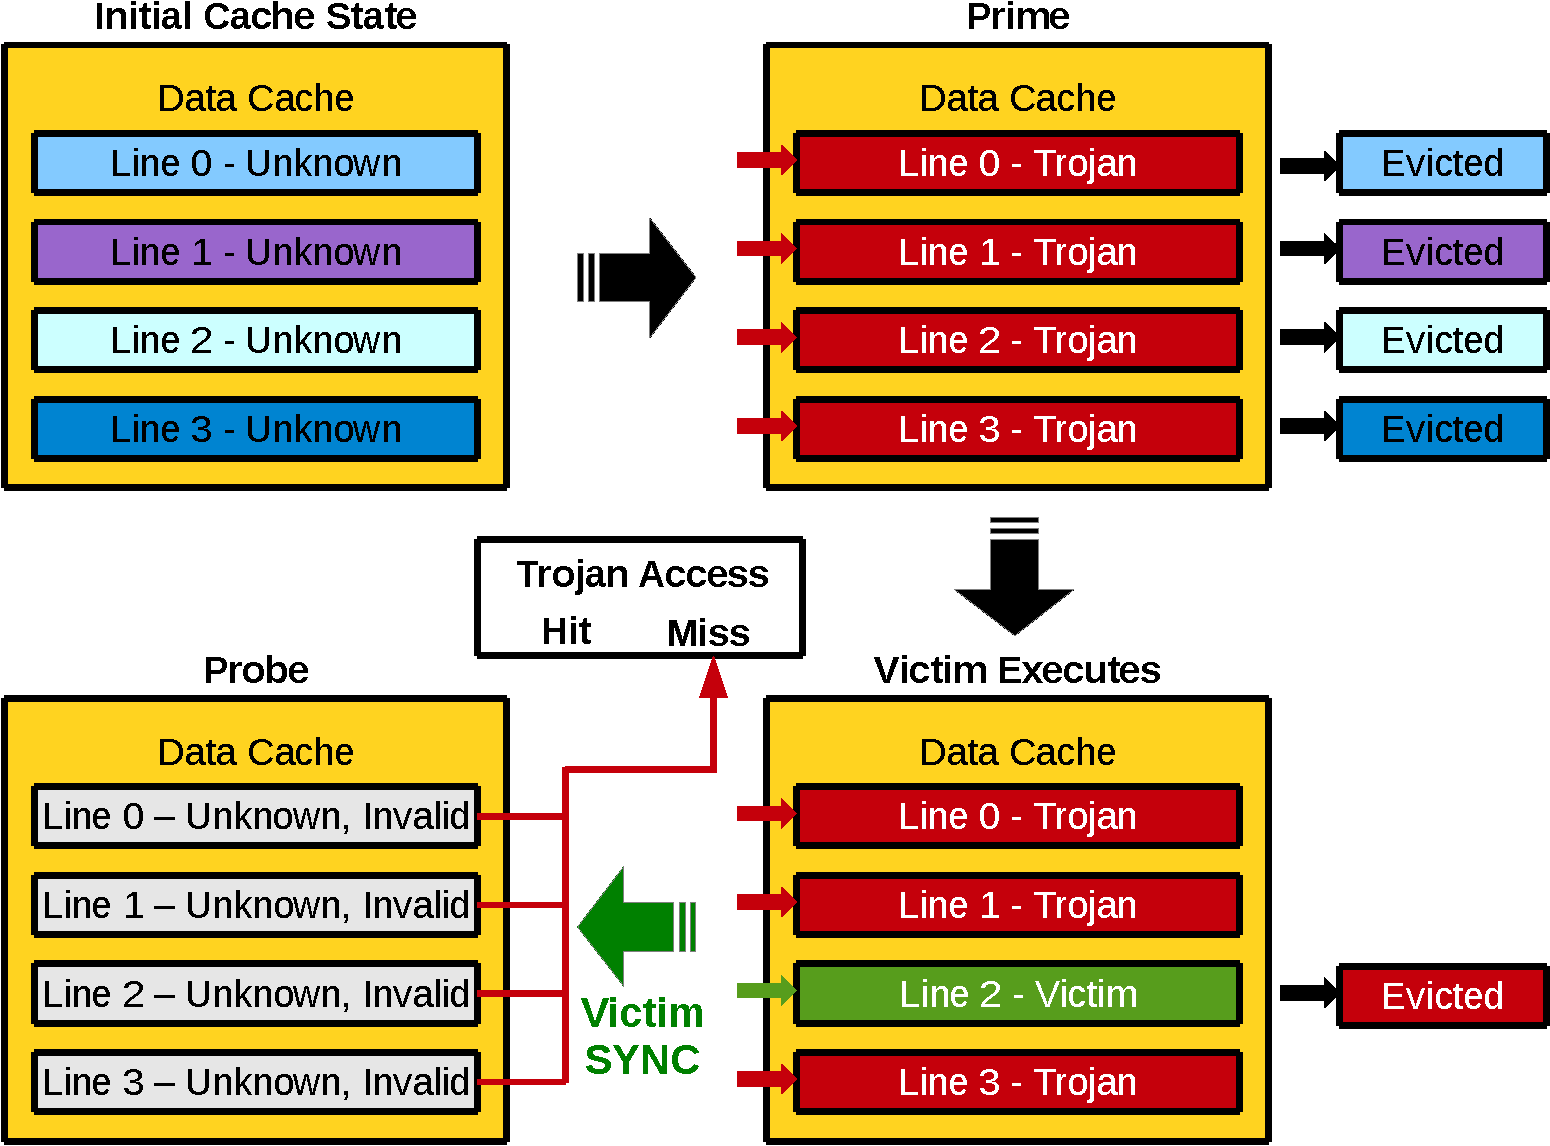
\includegraphics[width=\textwidth,height=\textheight,keepaspectratio]{prime_and_probe_time_based}}
				\caption{Prime+Probe attack, time-based coherence} 
				\label{prime_and_probe_time_based}
			\end{figure}
			%\vspace{-5mm}
			
			I have previously mentioned that time-based coherence does little to mitigate attacks on lower levels of memory, such as the shared cache. However, incorporating the single cycle flush mechanism may help. The shared cache tends to be much larger than the private caches, so purging cached data may degrade overall performance. These overheads could be reduced by flushing data only when the Victim application completes or during a context switch. Systems using three levels of cache could benefit from this mechanism at levels 1 and 2, but level 3 cache purging may be too costly. Attacks on level 3 caches have been demonstrated and SCA protection at this level will likely require one of the techniques suggested in \cite{Irazoqui15,Yarom14,Hund13,Brumley11}.
	
	\section{Experimental Set-up}
		In this section evaluate the level of SCA mitigation provided by time-based coherence. The memory footprint of a simple application is estimated through a cache side-channel. In order to simplify the analysis of the timing data and remove any unexpected noise due to other data in the cache, the  critical application or Victim is a simple loop containing memory load and store operations. Test simplicity and lack of external factors, greatly improve chances of a successful SCA. 
		
		The Trojan program consists of two array manipulation loops: Prime and Probe. The Prime loop loads a data cache sized array and stores it repeatedly in a volatile variable. This ensures that the operation is not optimised away by the compiler. The loaded value is updated and stored back into the cache. The Probe phase simply loads all previously ``primed'' data and measures the execution time of the loop. Any fluctuations in total time will reveal the hit-miss ratio. The Prime+Probe attack is applied to the entire BERI data cache (16KB, 32 bytes per line, 512 lines). The test yields very precise results in a controlled bare metal Bluesim environment. 

		%\textcolor{red}{However, when testing with an OS, such a measurement style suffers from noise due to other programs. Testing under FreeBSD on FPGA yields far more erratic results, but more timing samples allow us to conduct a successful SCA.} 
		SCA testing on FreeBSD OS is noisier and requires more Probe samples, I do not block other processes or interrupts during the test. The main test objective is to establish any SCA masking effects provided by the cache, so the same level of time sampling is applied to all designs under tests.
		
		\begin{enumerate}
			\item Prime: The Trojan populates the entire data cache with its data.
			\item Victim: The Victim program is allowed to execute. This program loads and stores chunks of memory. The size of this memory can be adjusted. A larger chunk of memory would result in more Trojan data evictions from the data cache.
			\item Probe: The Trojan loads all of its data and measures the execution time of the loop.
		\end{enumerate}
		
		The BERI data cache used in this evaluation is 16KB in size with 32 bytes per line. In order to reduce the execution time of the Trojan, the program only loads and stores every 32\textsuperscript{nd} byte of its memory chunk. This ensures that each data cache line will contain at least one byte of Trojan data. The exact placement of the Trojan byte within the line is irrelevant, as any other memory access to this line will cause a miss due to mismatched Tags, resulting in Trojan data eviction.
		
		This test also operates at the granularity of an L2 cache; the Trojan populates the shared cache but the Victim dataset is still limited to the L1 data cache size. In most cases the best Trojan timing information is extracted when only the data cache is populated. Time-based coherence provides no protection for the shared cache since it has no control over L2 evictions. Side channel attacks on shared caches are discussed further in Section \ref{protecting_llc}.
	
	\section{Bare Metal Testing}
		In the bare metal environment (\textit{i.e.} no OS) we have access to all hardware counters that may be restricted to kernel space. Counters are read through coprocessor 0 (CP0) using the read hardware register (RDHWR) instruction. The data cache counters are fed into CP0 every cycle. Counters used in this evaluation are:
		
			\begin{itemize}
				\item \textbf{Time:} This counter follows the standard MIPS model and provides a cycle-accurate count.
				\item \textbf{Miss:} Total data cache misses, including both loads and stores.
				\item \textbf{Hit:} Total data cache hits, including both loads and stores.
			\end{itemize}
	
		\subsection{Collocated Tests}
			Multiprocessor systems allow application parallelism, an important consideration when it comes to memory side-channel evaluation. Many SCAs rely on the Trojan and the Victim application to be collocated, that is, sharing the same private cache. This test evaluates an SCA on a Victim application where both are executed on the same core. On BERI, the Trojan and Victim codes are tied to core 0. Core affinity is assured by locking Core 1 in an infinite loop, so that minimal interference is expected.

\begin{comment}
\url{Location: /home/aam53/TestsForMIPSResults/BaremetalTestResults/20151106_baremetal_core_pin/*}
\end{comment}

			\subsubsection{Results}
				The Victim code operates on a dataset with a memory size ranging from 0 bytes to a maximum of 16,384 bytes (maximum data cache capacity). The memory usage of the Victim is increased every test iteration in order to determine the amount of side-channel leakage. The test gathers the following processor statistics for each memory test size: (1) Trojan Probe time, (2) Trojan Probe miss count, (3) Trojan Probe hit rate, and (4) Victim execution time.
				
				\paragraph{Expected Behaviour}
					The initial cache state is irrelevant, so the Trojan begins the Prime phase by reading in uninitialised data and updating it to a known value. The Trojan is only interested in timing measurements but initialising the data is useful for debugging. BERI data caches are non write-allocate, loads ensure subsequent caching of stores. Each cache line holds 32 bytes of data and it is sufficient for the Trojan to only touch every 32\textsuperscript{nd} byte of its data. A total of 512 loads and 512 stores are performed in the Prime phase.
					
					Following the Prime operation, core 0 begins executing the Victim code. This code consecutively loads bytes, increments their value, and then stores them back into the cache. The load operation is sufficient to evict a Trojan line but the increment operation is added to simulate some kind of useful work. It isn't a memory operation so it simply passes through the pipeline, spacing out memory accesses.
					
					Once the Victim completes its execution, the Trojan begins the Probe phase. Counter values are acquired and stored in specific memory locations. The Trojan performs 512 load operations. Any data not present in the data cache will result in a miss and an access to the L2 or main memory, this generates additional latency and a slower execution of the Probe phase. 
					On completion, the counters are read again and the difference between initial and final values provide the required information. Note that several unrelated memory accesses due to counter loading are acknowledged in the final count, the added error is minuscule and does not show a significant impact on the overall results.
					
					The Victim dataset size is determined through time-counter values and reinforced by other counters. Timing data gathered by the Trojan can precisely identify the Victims memory footprint. Timing results are also supported by capturing hit and miss counters, thus verifying Trojan and Victim behaviour.
				
				\paragraph{Observed Behaviour - Single-Core}
					In the bare metal environment, the single-core Trojan and Victim behaviour is almost identical to that shown by the directory. The absence of a coherence network reduces any coherence noise that may be present in the directory version. Given the similarity in observations, we will discuss these in the directory section below.
				
				\paragraph{Observed Behaviour - Directory}
					As expected in a processor with no side-channel mitigation and Trojan-Victim collocation, the Probe observations are highly deterministic and perfectly correlate with variations in the Victim's dataset size. 
					The size is directly proportional to the execution time and miss rates of the Trojan Probe phase, the hit rate of Trojan Probe data is inversely proportional to the Victim dataset size. 
					No data sharing is expected, so any coherence messages observed in the cache are due to L2 cache capacity misses. Trojan observations are limited to the line granularity of the cache. BERI caches use 32 bytes per line, any Victim dataset variations below that threshold are non-observable.
					
					The normalised 2D cross-correlation function in Matlab calculates the correlation coefficients of the two inputs; the array of Victim datasets and the array of Trojan Probe execution times. The result shows a sharp peak centred around 1 where the two data sequences show maximum correlation.
				
				\paragraph{Observed Behaviour - Time-Based}
					%\textcolor{red}{Trojan observations are dramatically different in the time-based system. The Probe phase execution time and hit/miss rates are very noisy. Additionally the miss rate is much higher since the Trojan data has been self-invalidated from the data cache. The hit rate is equally chaotic. The correlation chart shown no peaks since there is no correlation between the Trojan time data and the Victim dataset size.}
					
					The Trojan Probe samples little to no correlation with the Victims dataset size. Some side-channel leakage is observable when the Victim execution time is low, however, the obtained results are insufficient for accurately identifying the Victims memory usage. The miss and hit counts are very different to those shown by the single-core or dual-core directory systems. While some similarity is visible, the number of matching samples is low. The timing charts shown in this section may be visually deceptive as some samples overlap, the cross-correlation charts show a more accurate data representation.
				
			\subsubsection{Evaluation}
				Data gathered from the SCA simulation test is shown and discussed in this section. Each cluster of plots is discussed separately.
			
				\paragraph{Figure \ref{baremetal_core_pin_std_1} --}
					The data presented in this figure shows the relation between the Victim process and any side-channel data extracted by the Trojan application. 
					\begin{description}
					\item [a(1,2,3)] 
						We observe a linear relation between the execution time of the Victim application and its dataset size for all three models. Crucially, time-based coherence behaviour for the Victim application is nearly identical. Thus, any side-channel masking offered by time-based coherence does not negatively impact the Victim application.
					\item [b(1,2,3)] 
						When we zoom in to the a(1,2,3) data, we see that single-core and dual-core directory models display identical Victim behaviour. Time-based coherence b(3) follows the same general pattern with occasional high latency samples due to time-counter roll-overs in the L1 data cache. Approximately 11\% of all Victim executions suffer from these performance penalties.
					\item [c(1,2,3)] 
						This chart analyses latency experienced by the Trojan Probe for each Victim dataset size. The single-core and directory designs both show a linear relationship between the two chart parameters. This result follows the expected behaviour of a system lacking SCA protection. The Victim test code does not use any software SCA mitigation techniques such as cache flushing, uncached accesses, etc.
						
						Trojan Probe execution measurements are dramatically different in the time-based results, the Trojan experiences almost no data cache hits and even shows L2 cache misses. The Victim program runtime affects the total time between the Prime and Probe stages, since time-based coherence self-invalidates data at fixed times, a greater Victim runtime results in a lower Trojan hit rate. This test shows that the Probe phase does not provide any meaningful results even at low Victim execution times. The time-based model used in this test has a fixed time offset value of 10,000 cycles. Once the execution time of the Victim exceeds 10,000 cycles, the data cache no longer holds any valid Trojan data. 
						%Lower execution times result in some side-channel leakage that is more visible in the next chart described below.
					\item [d(1,2,3)] 
						Looking at a region of charts c(1) and c(2) produces the patterns shown in d(1) and d(2). While data in c(1) and c(2) appears as a straight line, in reality the time values form more of a staircase pattern. Each step shows 32 identical time samples values followed by a jump to a new time value. This is due to bytes per line timing granularity, since 32 data bytes are located within a cache line. The Trojan can only observe latency at a line granularity. Both dual-core directory and single-core show identical behaviour.
						
						The time-based model shows a high fluctuation in latency. The staircase pattern is not observable in this data. The time-based model displays a much greater overall latency (y-axis minimum and maximum) in this window. Note that the high rate of variation in the Trojan measurement is present even for very small Victim execution times, and even when there is no Victim data. The Trojan Prime phase takes a certain amount of time to complete, and by the time it has finished, some of the lines written at the beginning might be near the end of their lifespan. For this reason, the Trojan might experience high memory latency even at low Victim execution rates.
					\end{description}
				
				\paragraph{Figure \ref{baremetal_core_pin_std_2x} --}
					In this chart we look at the cache hit, miss and correlations for the Trojan-Victim test.
					\begin{description}
					\item [a(1,2,3)] 
						The single-core and dual-core directory models follow the same pattern. The number of cache hits decreases proportionally with the increase in Victims dataset size. This behaviour is expected judging by the timing data displayed in the previous chart. 
						The Minimum cache hit of 0 is observed when the Victim fills the entire cache (16384 bytes) and the maximum cache hit of 512 is achieved when the Victims dataset size is 0. The Trojan only requires 512 memory accesses to touch every data cache line. 
						
						The time-based model shows an erratic cache hit behaviour. The number of hits is variable and often near 0 even when the Victim size is 0 (time-counter roll-overs may occur during the Prime phase). Hits significantly reduce once the Victim size exceeds the time-counter roll over threshold, 4 bit counter with a 10,000 cycle timing offset, a total of 160,000 cycles. Note that each memory operations will require multiple cycles to complete. In the previous Figure \ref{baremetal_core_pin_std_1}, charts a(1,2,3) show that the Victims execution time exceeds 160,000 cycles 
						\footnote{The time-counter continues incrementing through the Trojan Prime phase, and these cycles must be added to the Victims execution time. For this reason the sharp drop in Probe hit rate is observed when the Victims dataset size is at $\sim$11,000.}
						when the dataset size is $\sim$12,000. This directly translates to the sudden drop in hit rate experienced by the time-based model in a(3).
					\item [b(1,2,3)] 
						Miss count for all charts is inversely proportional to the corresponding hit rate, discussed above. This property holds for the entire range of the Victim dataset.
					\item [c(1,2,3)] 
						Data presented so far has shown a clear distinction between different model behaviours. Correlations between the Victim and Trojan results are easy to visualise. However, if the Victim dataset size is randomly varied, it may be more difficult to visually identify correlations. Hence, data presented in charts c(1,2,3) and d(1,2,3) quantifies the results using a normalised cross-correlation function. This technique should consistently identify any correlation between the Victim and Trojan behaviour. The single-core and directory correlations are identical as the input data is effectively the same. We see a strong peak where the cross-correlation of the Victims dataset size and Trojans Probe timing yields maximum similarity. The time-based model shows no correlation whatsoever.
					\item [d(1,2,3)]
						Here we look at the cross-correlation between the acquired hit and miss counts for all the models. Since cache hit and miss counts are inversely proportional for both single-core and directory, a strong inverse peak is observed. A minor correlation is also observable in the time-based data comparison. If the cache miss/hit data were to be available to an attacker, useful information could still be extracted when using the time-based model.
					\end{description}

% Figure batch 1
					\begin{figure}[!h]
					\centering 
						\makebox{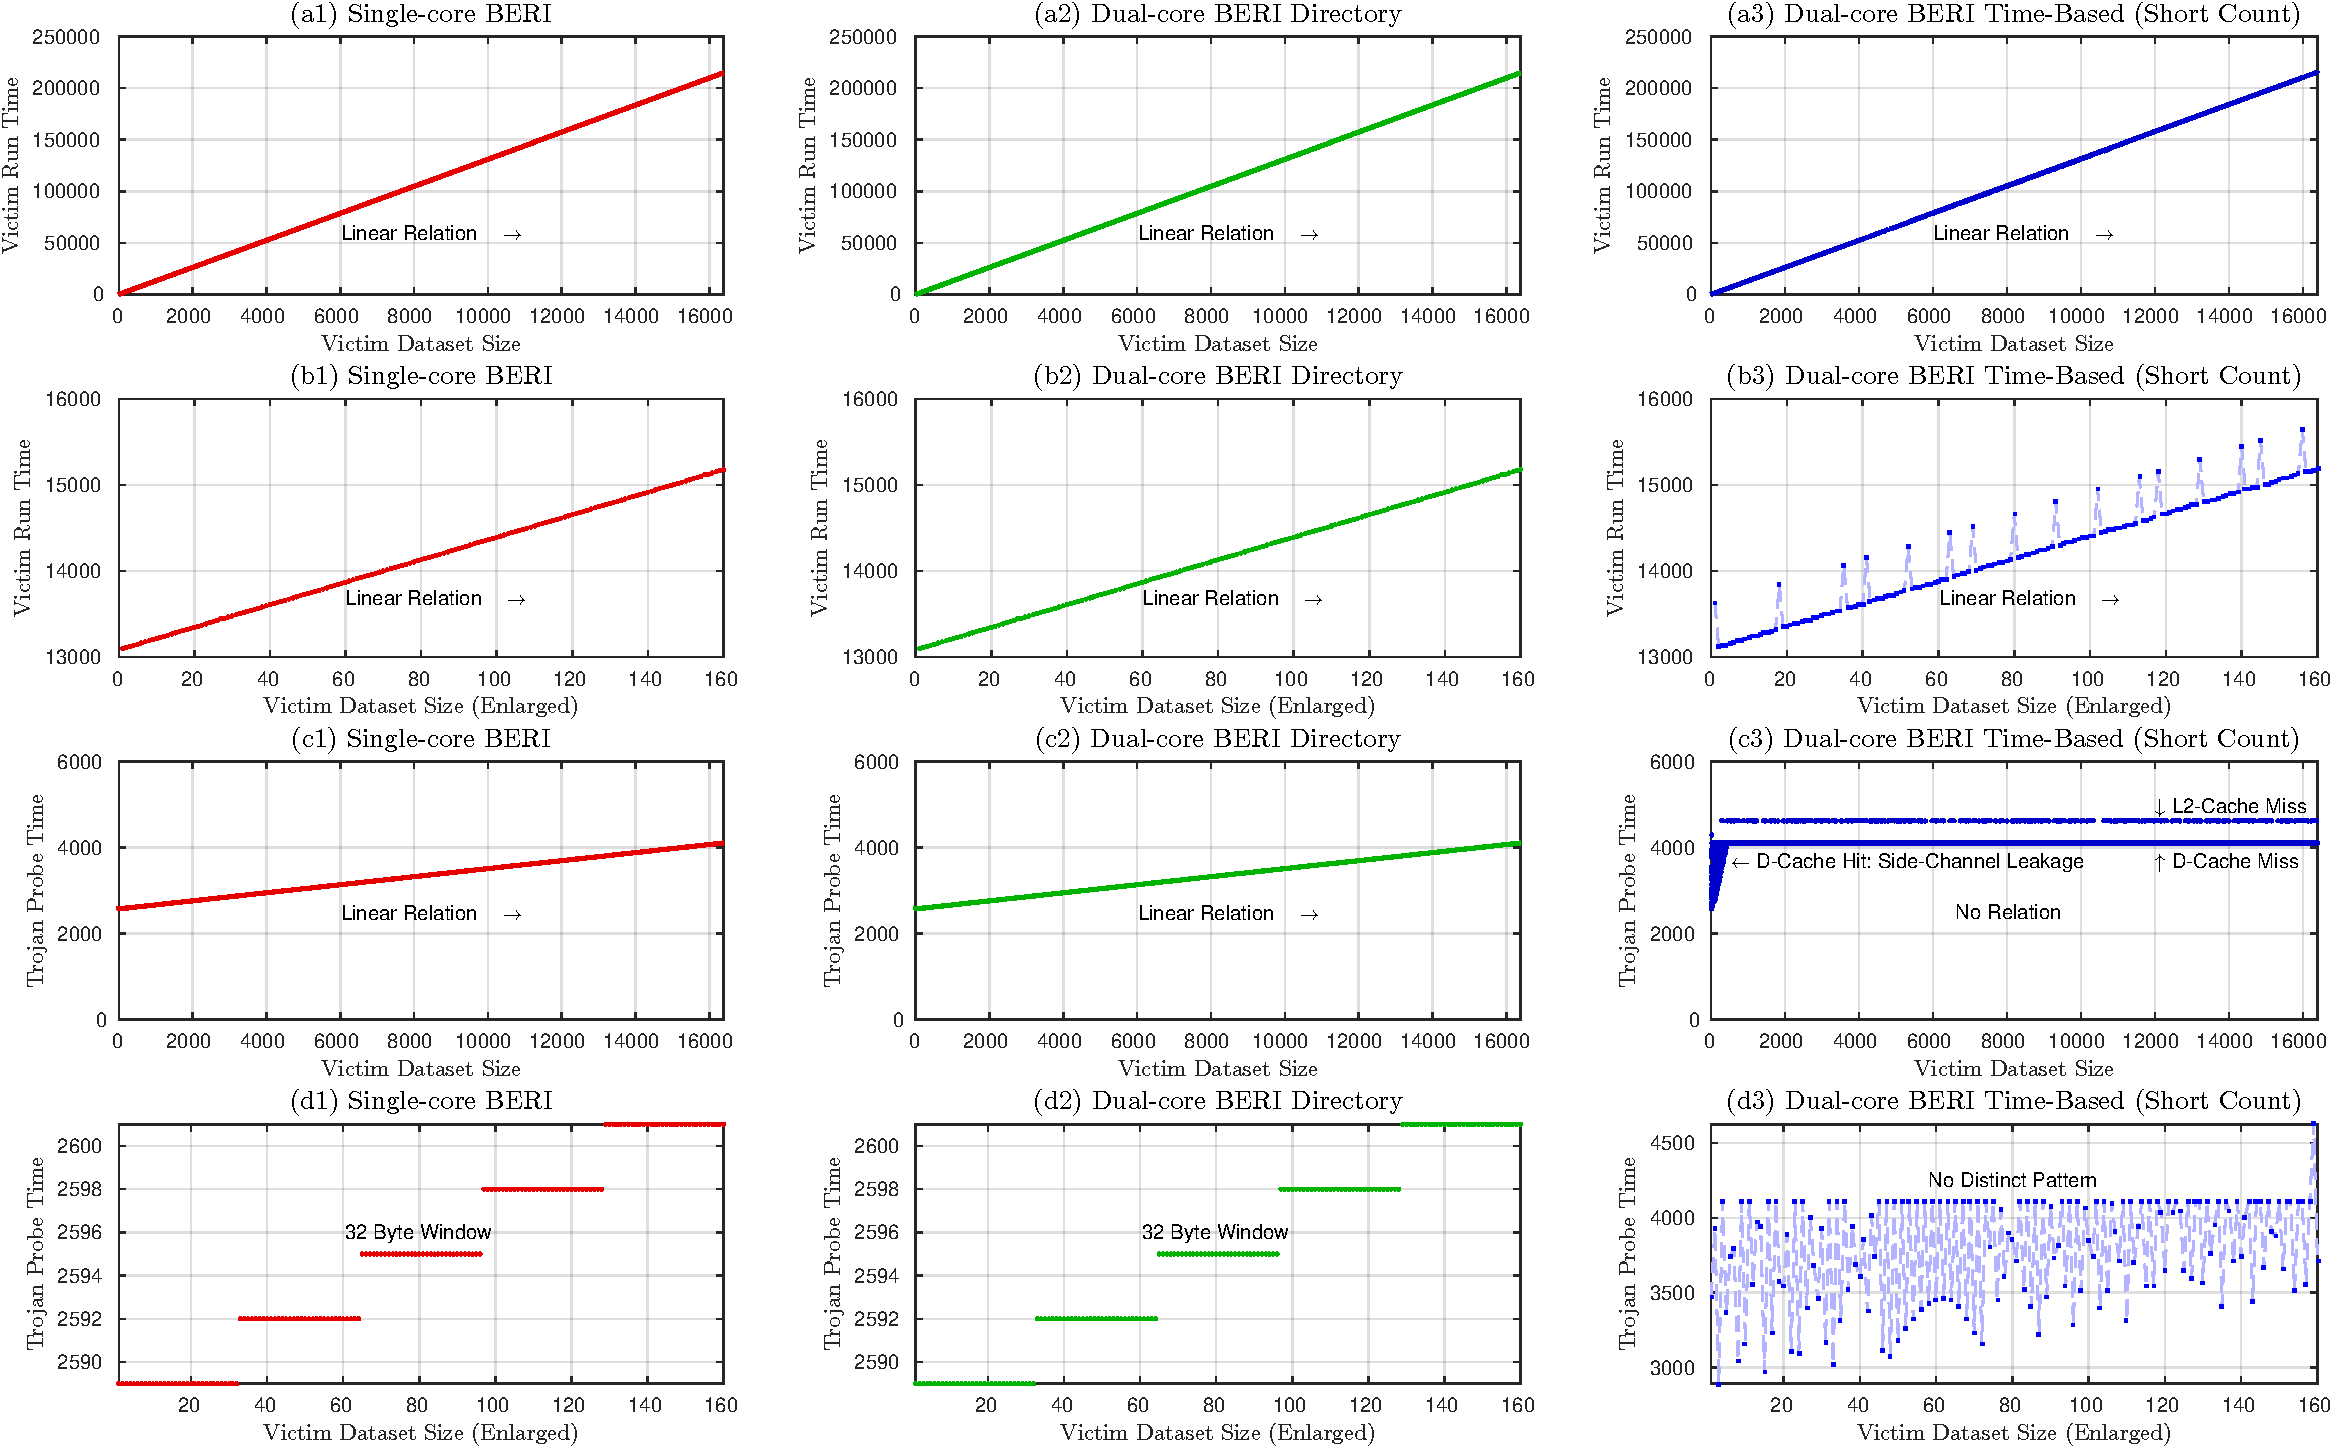
\includegraphics[width=\textheight,height=0.95\textwidth,keepaspectratio,angle=90]{sca_baremetal_standard_1}}
						\caption{Bare metal side-channel attack, chart (1a)} 
						\label{baremetal_core_pin_std_1}
					\end{figure}
					
					\begin{figure}[!h]
					\centering 
						\makebox{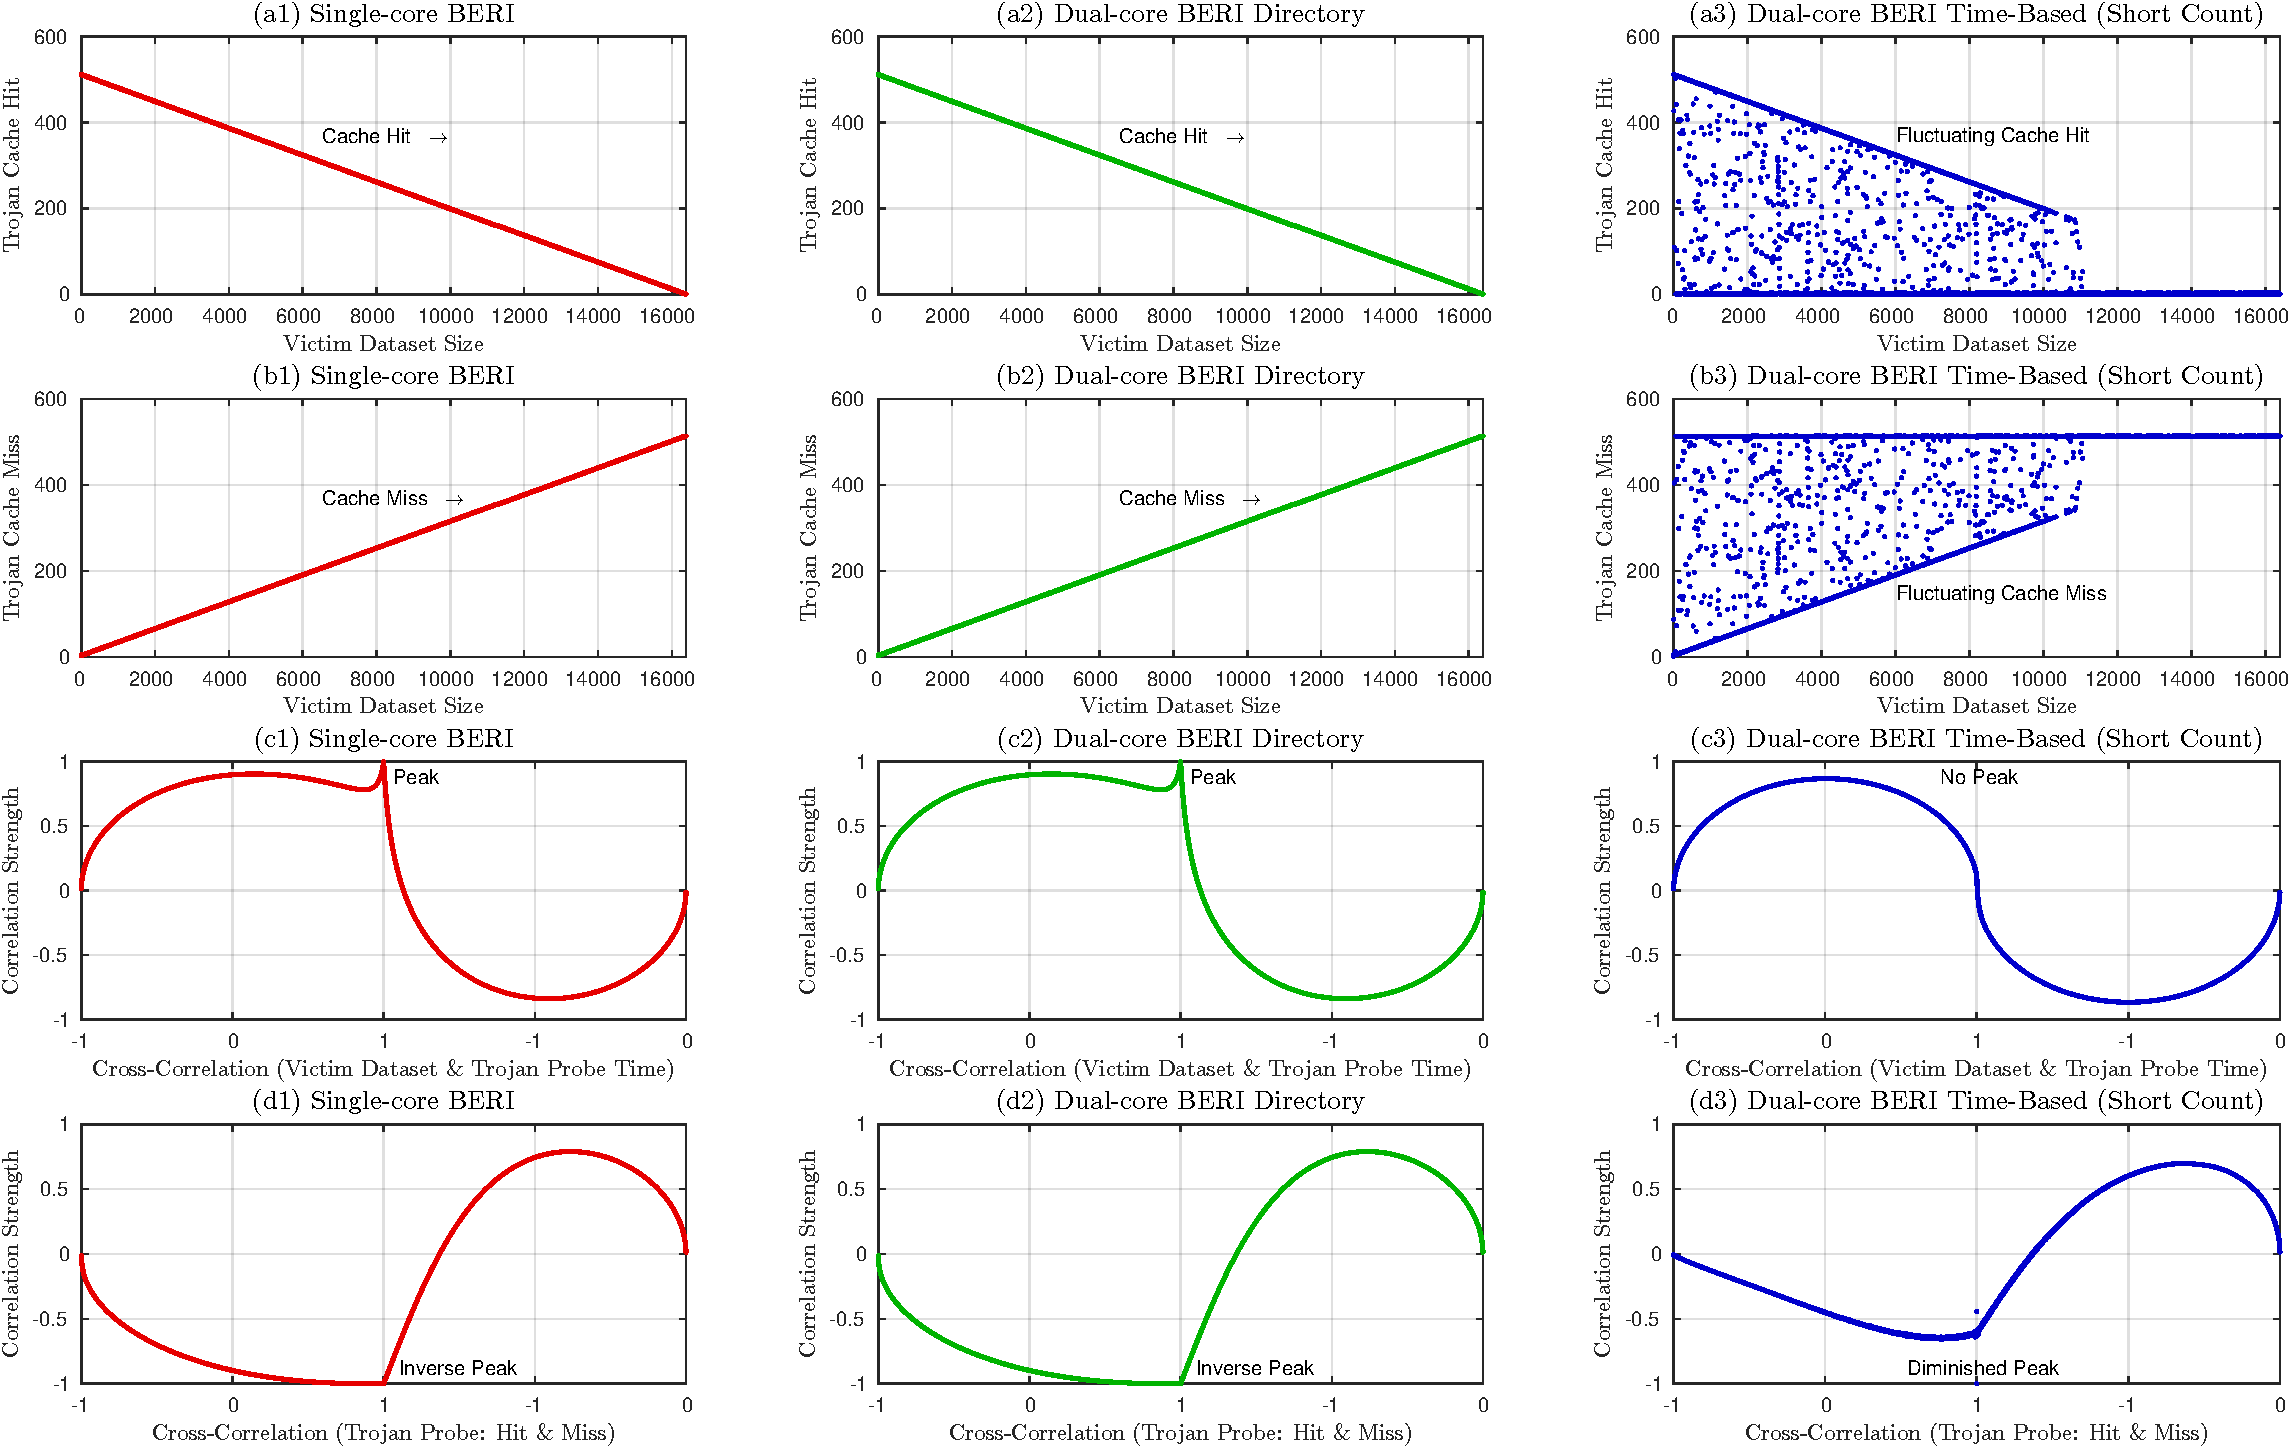
\includegraphics[width=\textheight,height=0.95\textwidth,keepaspectratio,angle=90]{sca_baremetal_standard_2x}}
						\caption{Bare metal side-channel attack, chart (1b)} 
						\label{baremetal_core_pin_std_2x}
					\end{figure}
			


\clearpage
				\paragraph{Figure \ref{baremetal_core_pin_long_1} --}
						In this figure we look at the side-channel leakage of a time-based coherence scheme using a long counter offset (100,000 cycles). Results for the directory scheme and the time-based model using a short counter offset (10,000 cycles) have already been discussed in Figures \ref{baremetal_core_pin_std_1} and \ref{baremetal_core_pin_std_2x}. They are used as a reference to highlight any additional side-channel leakage that may be produced by a less-aggressive self-invalidation scheme.
					\begin{description}
					\item [a(1,2,3)] 
						All models show a similar Victim execution time for a given dataset size.
					\item [b(1,2,3)]
						Charts a(1,2,3) are enhanced to highlight any fluctuations in the Victims execution time. The long counter offset time-based model  shows fewer time-counter overflows, as a result, only $\sim$1\% of all Victims code iterations show a slower execution time. Compared with the short counter model, the overall performance penalty caused by self-invalidates is significantly reduced. These results match the Splash-2 benchmark observations.
					\item [c(1,2,3)]
						Data shown in c(1) and c(2) has been previously discussed. The long counter scheme (shown in c(3)) preserves cached data for a longer time duration; thus, showing more side-channel leakage. The ideal leakage plot shows the expected outcome for a system without SCA protection, such as the directory model. The time-based model still offers some side-channel masking, but the leakage shown is sufficient for extracting useful information. Any Victim application with an execution time of 100,000 cycles or less will be compromised. 
						
						This example clearly shows that selecting a time-count offset is critical for SCA mitigation. I have already mentioned that inserting a SYNC instruction just after the Victims execution will be sufficient to mask side-channel leakage, this property holds for all offset values. If a SYNC instruction had been adequately used in this test, we would observe consistent data cache misses during the Trojan Probe phase.
					\item [d(1,2,3)] 
						Since the granularity of cache access timing is restricted to 32 bytes, we continue seeing the stepped pattern for the directory case. Note that the scale used to display charts d(1)--d(3) is identical, and the time-based short counter offset scheme does not show any samples in this range due aggressive cache self-invalidations. The pattern shown by the long count version is much closer to that shown by the directory model, but the time-based model still experiences a regular pattern of high latency. The noise is sufficiently low, allowing the attacker to extract useful information.
					\end{description}
				
				\paragraph{Figure \ref{baremetal_core_pin_long_2x} --}
					In this figure we look at the cache hit and miss count, as well as the correlation between data captured by the Trojan and known Victim behaviour.
					\begin{description}
					\item [a(1,2,3)] 
						Comparing the two time-based models we see that the long count version provides cleaner cache hit samples. While this data is not identical to the directory behaviour, we can observe a matching pattern. Unlike the short counter version, we do not observe a sharp drop-off in hits. The long count version experiences roll-overs 10 times less frequently.
						The Victims execution time never exceeds 250,000 cycles and the long timer offset model requires 1,600,000 (16$\times$100,000 cycles) cycles for a time-counter roll-over. 
						The counter roll-over is one of the major performance drawbacks of the time-based coherence model.
					\item [b(1,2,3)] 
						The observed miss counts are again inversely proportional to the corresponding hit counts and follow the expected behaviour. 
					\item [c(1,2,3)] 
						The previous set of results illustrated in Figures \ref{baremetal_core_pin_std_1} and \ref{baremetal_core_pin_std_2x}
						have established that the short counter time-based model does not demonstrate any correlation between the Trojan Probe data and the Victim behaviour. While the long counter model shows some correlation. However, when observing the full range of Victims data, a higher overall execution time will allow the time-based long counter to provide more side-channel masking.
					\item [d(1,2,3)]
						The correlation shown between the hit and miss count is significantly improved in the time-based long counter model. The purpose of this correlation is to identify any patterns in memory behaviour, this data is not normally available to the attacker. It also provides a good metric for comparing different versions of the SCA tests and time-based models.
					\end{description}
% Figure batch 2
					\begin{figure}[!h]
					\centering 
						\makebox{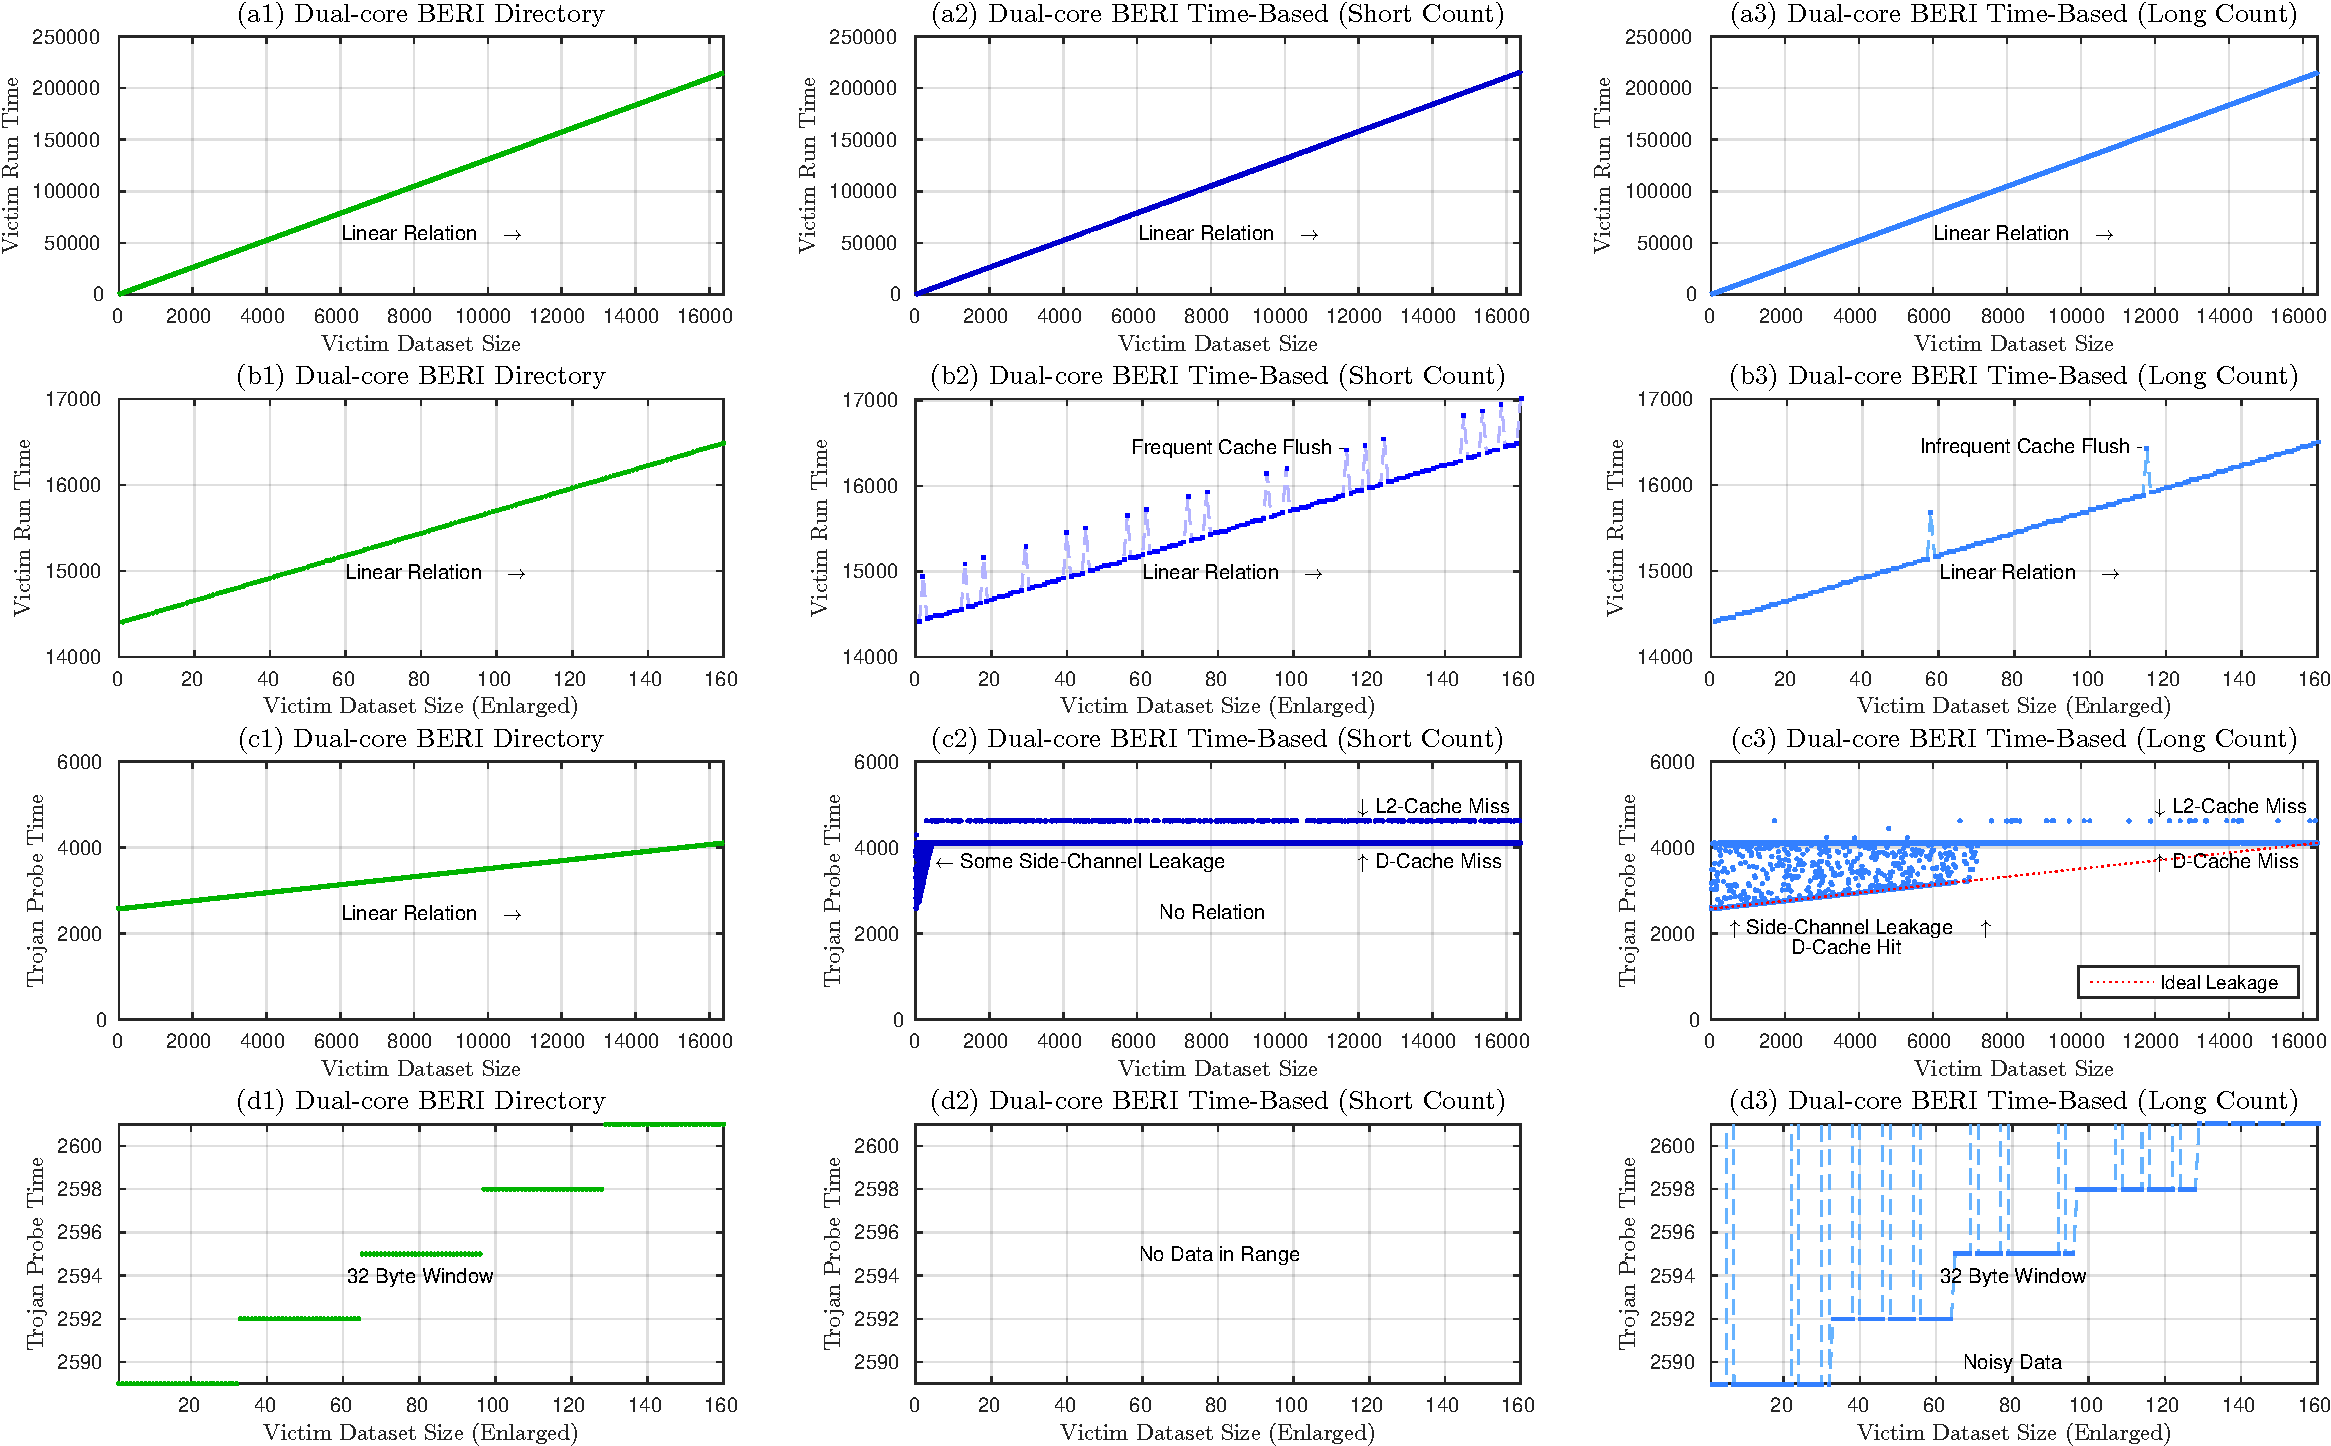
\includegraphics[width=\textheight,height=0.95\textwidth,keepaspectratio,angle=90]{sca_baremetal_long_1}}
						\caption{Bare metal side-channel attack, chart (2a)} 
						\label{baremetal_core_pin_long_1}
					\end{figure}
					
					\begin{figure}[!h]
					\centering 
						\makebox{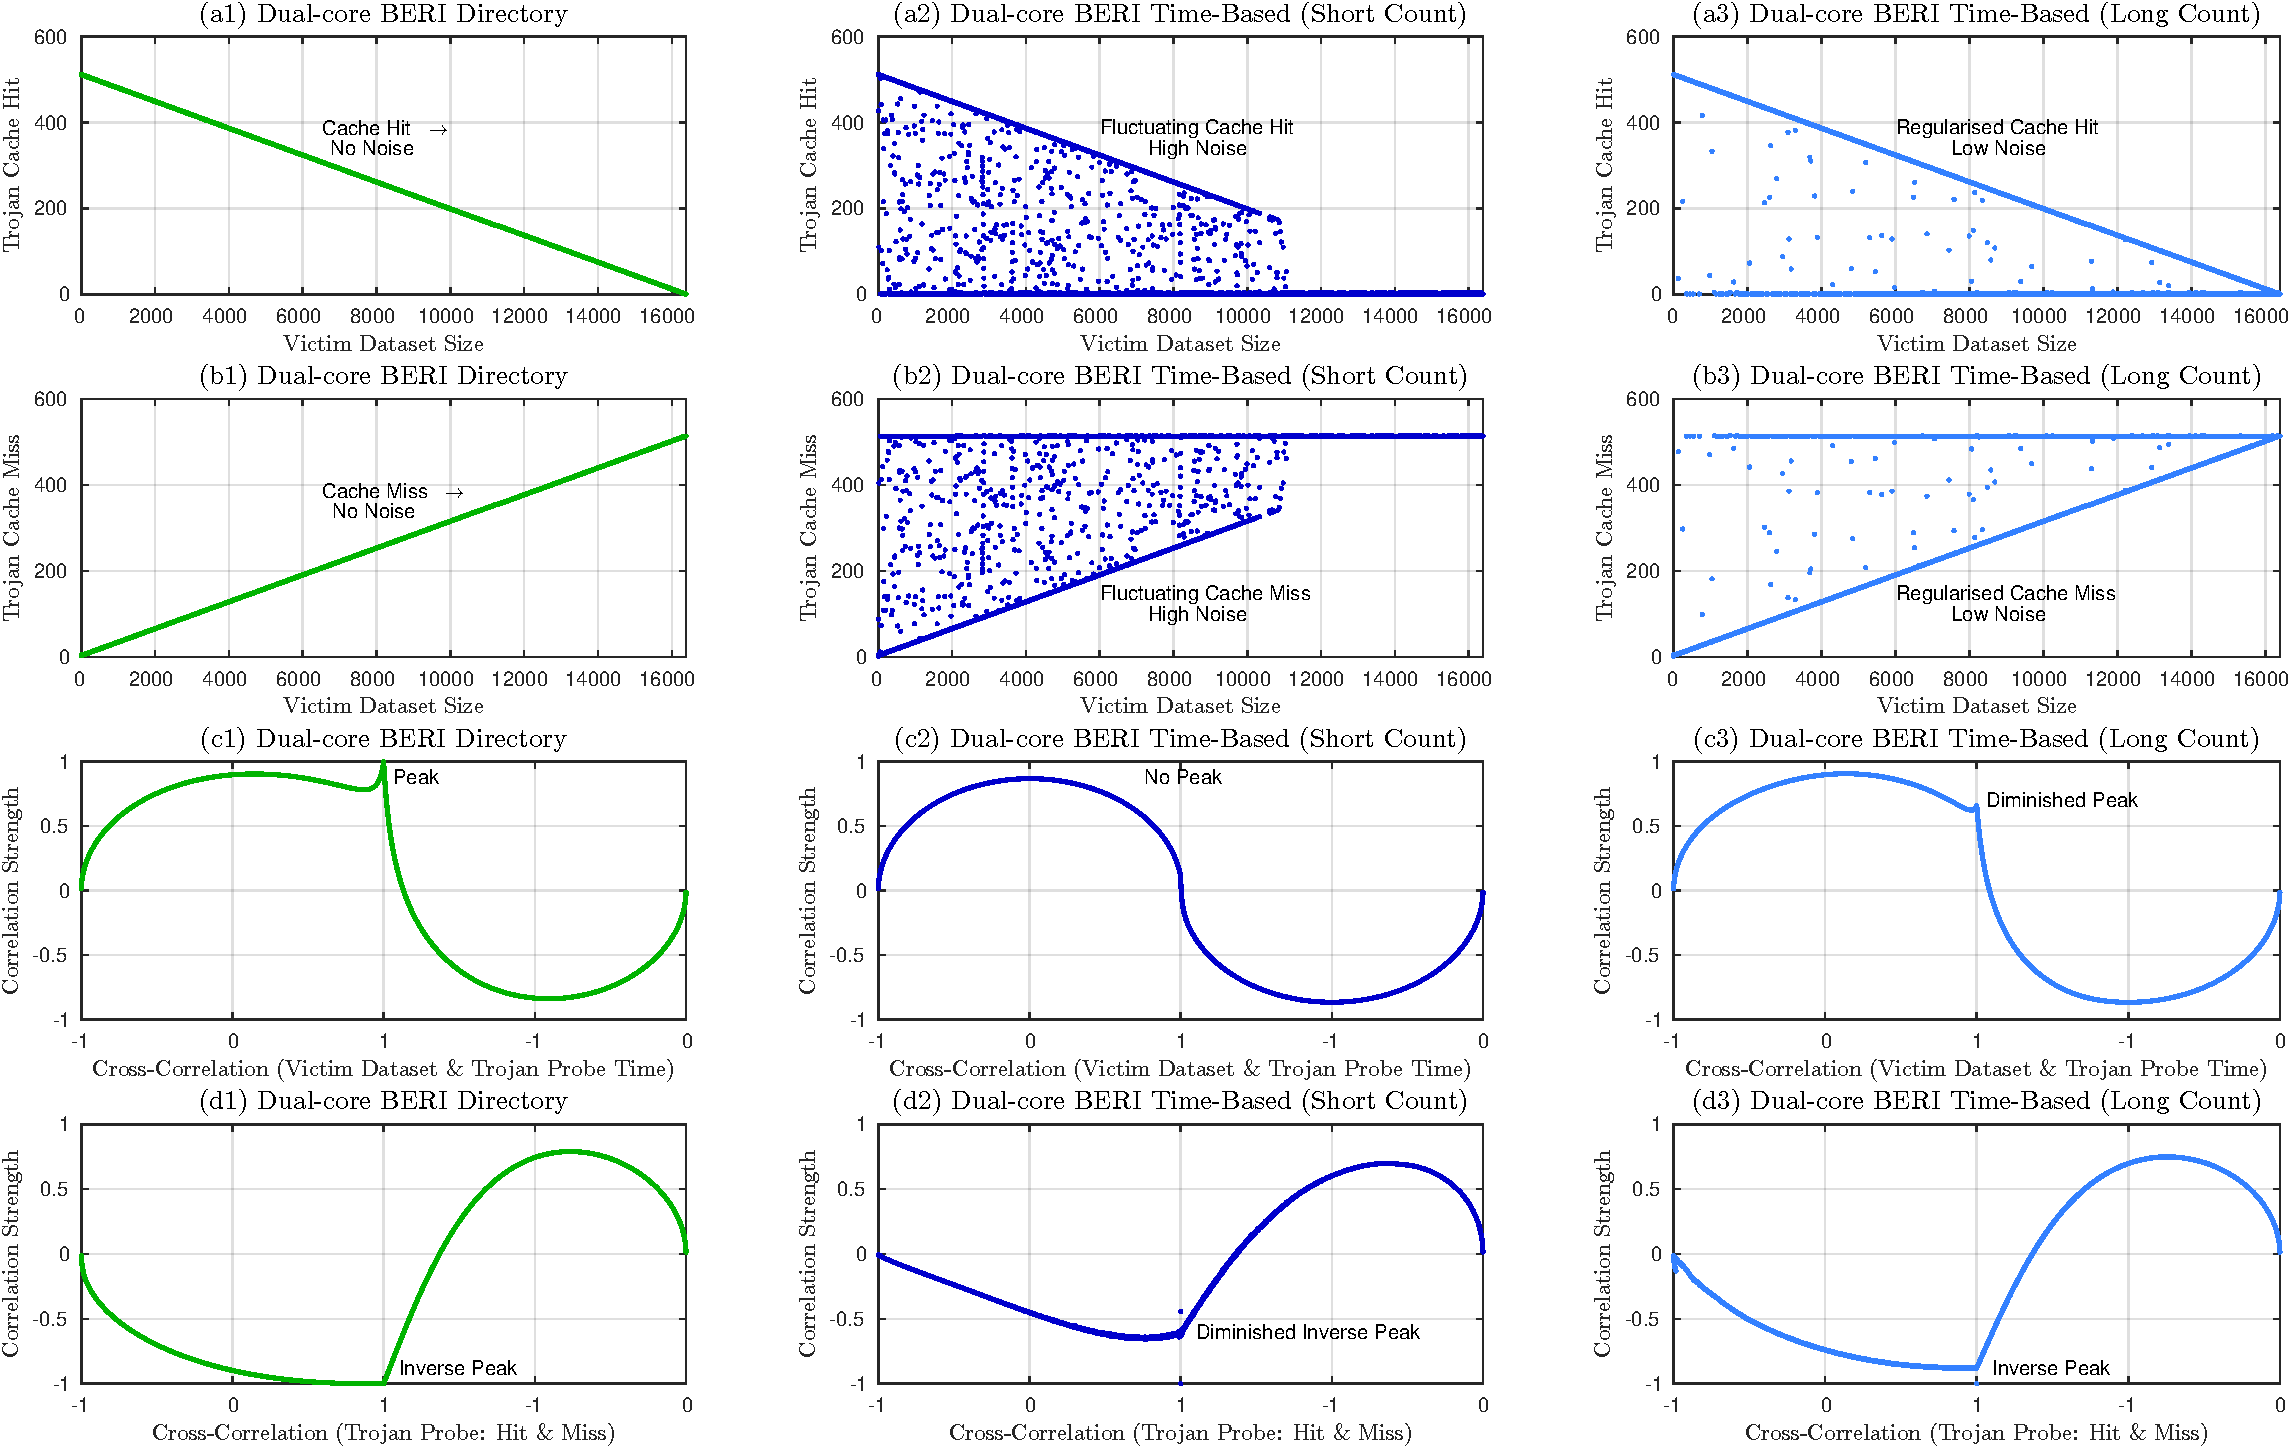
\includegraphics[width=\textheight,height=0.95\textwidth,keepaspectratio,angle=90]{sca_baremetal_long_2x}}
						\caption{Bare metal side-channel attack, chart (2b)} 
						\label{baremetal_core_pin_long_2x}
					\end{figure}


\clearpage
				\paragraph{Figure \ref{baremetal_core_pin_reverse} --}
					In the default SCA test, the Trojan Probe reads back data in the same ascending address order as the Prime phase. An attacker aware of the time-based coherence scheme may trick the system into leaking more side-channel information by probing data in a descending order (reverse test). 
					
					Most recent Trojan data is more likely to hold a valid tag-time-stamp, so evictions caused by the Victim could still be detected. The directory model is not displayed in this set of tests as the order of Probe acquisition makes no difference. Note that in this figure, data gathered for each model is displayed in rows, rather than columns. 
					\begin{description}
					\item [a(1,2,3)] 
						The default test running on the short count version shows minimal or no side-channel leakage. 
					\item [b(1,2,3)] 
						When the reverse test is executed on the short counter version, we observe a marginal increase in side-channel leakage. The timing data is very noisy, but cache hits and misses show a much clearer pattern than a(2) and a(3). 
					\item [c(1,2,3)] 
						The default test running on the long count version shows moderate side-channel leakage, sufficient to detect data usage by small Victim applications.
					\item [d(1,2,3)] 
						This test case shows by far the most side-channel leakage. The data is noisy but many samples fall under the ideal leakage curve. This test clearly shows that improving the attack technique could yield better Trojan results. 
						
						If the attack were to be conducted on a single memory line, sufficient sampling would result in a precise SCA. As mentioned before, the leakage can be eliminated by appropriately inserting a SYNC instruction or using a smaller counter offset. 
					\end{description}
% Figure batch 3
					\begin{figure}[!h]
					\centering 
						\makebox{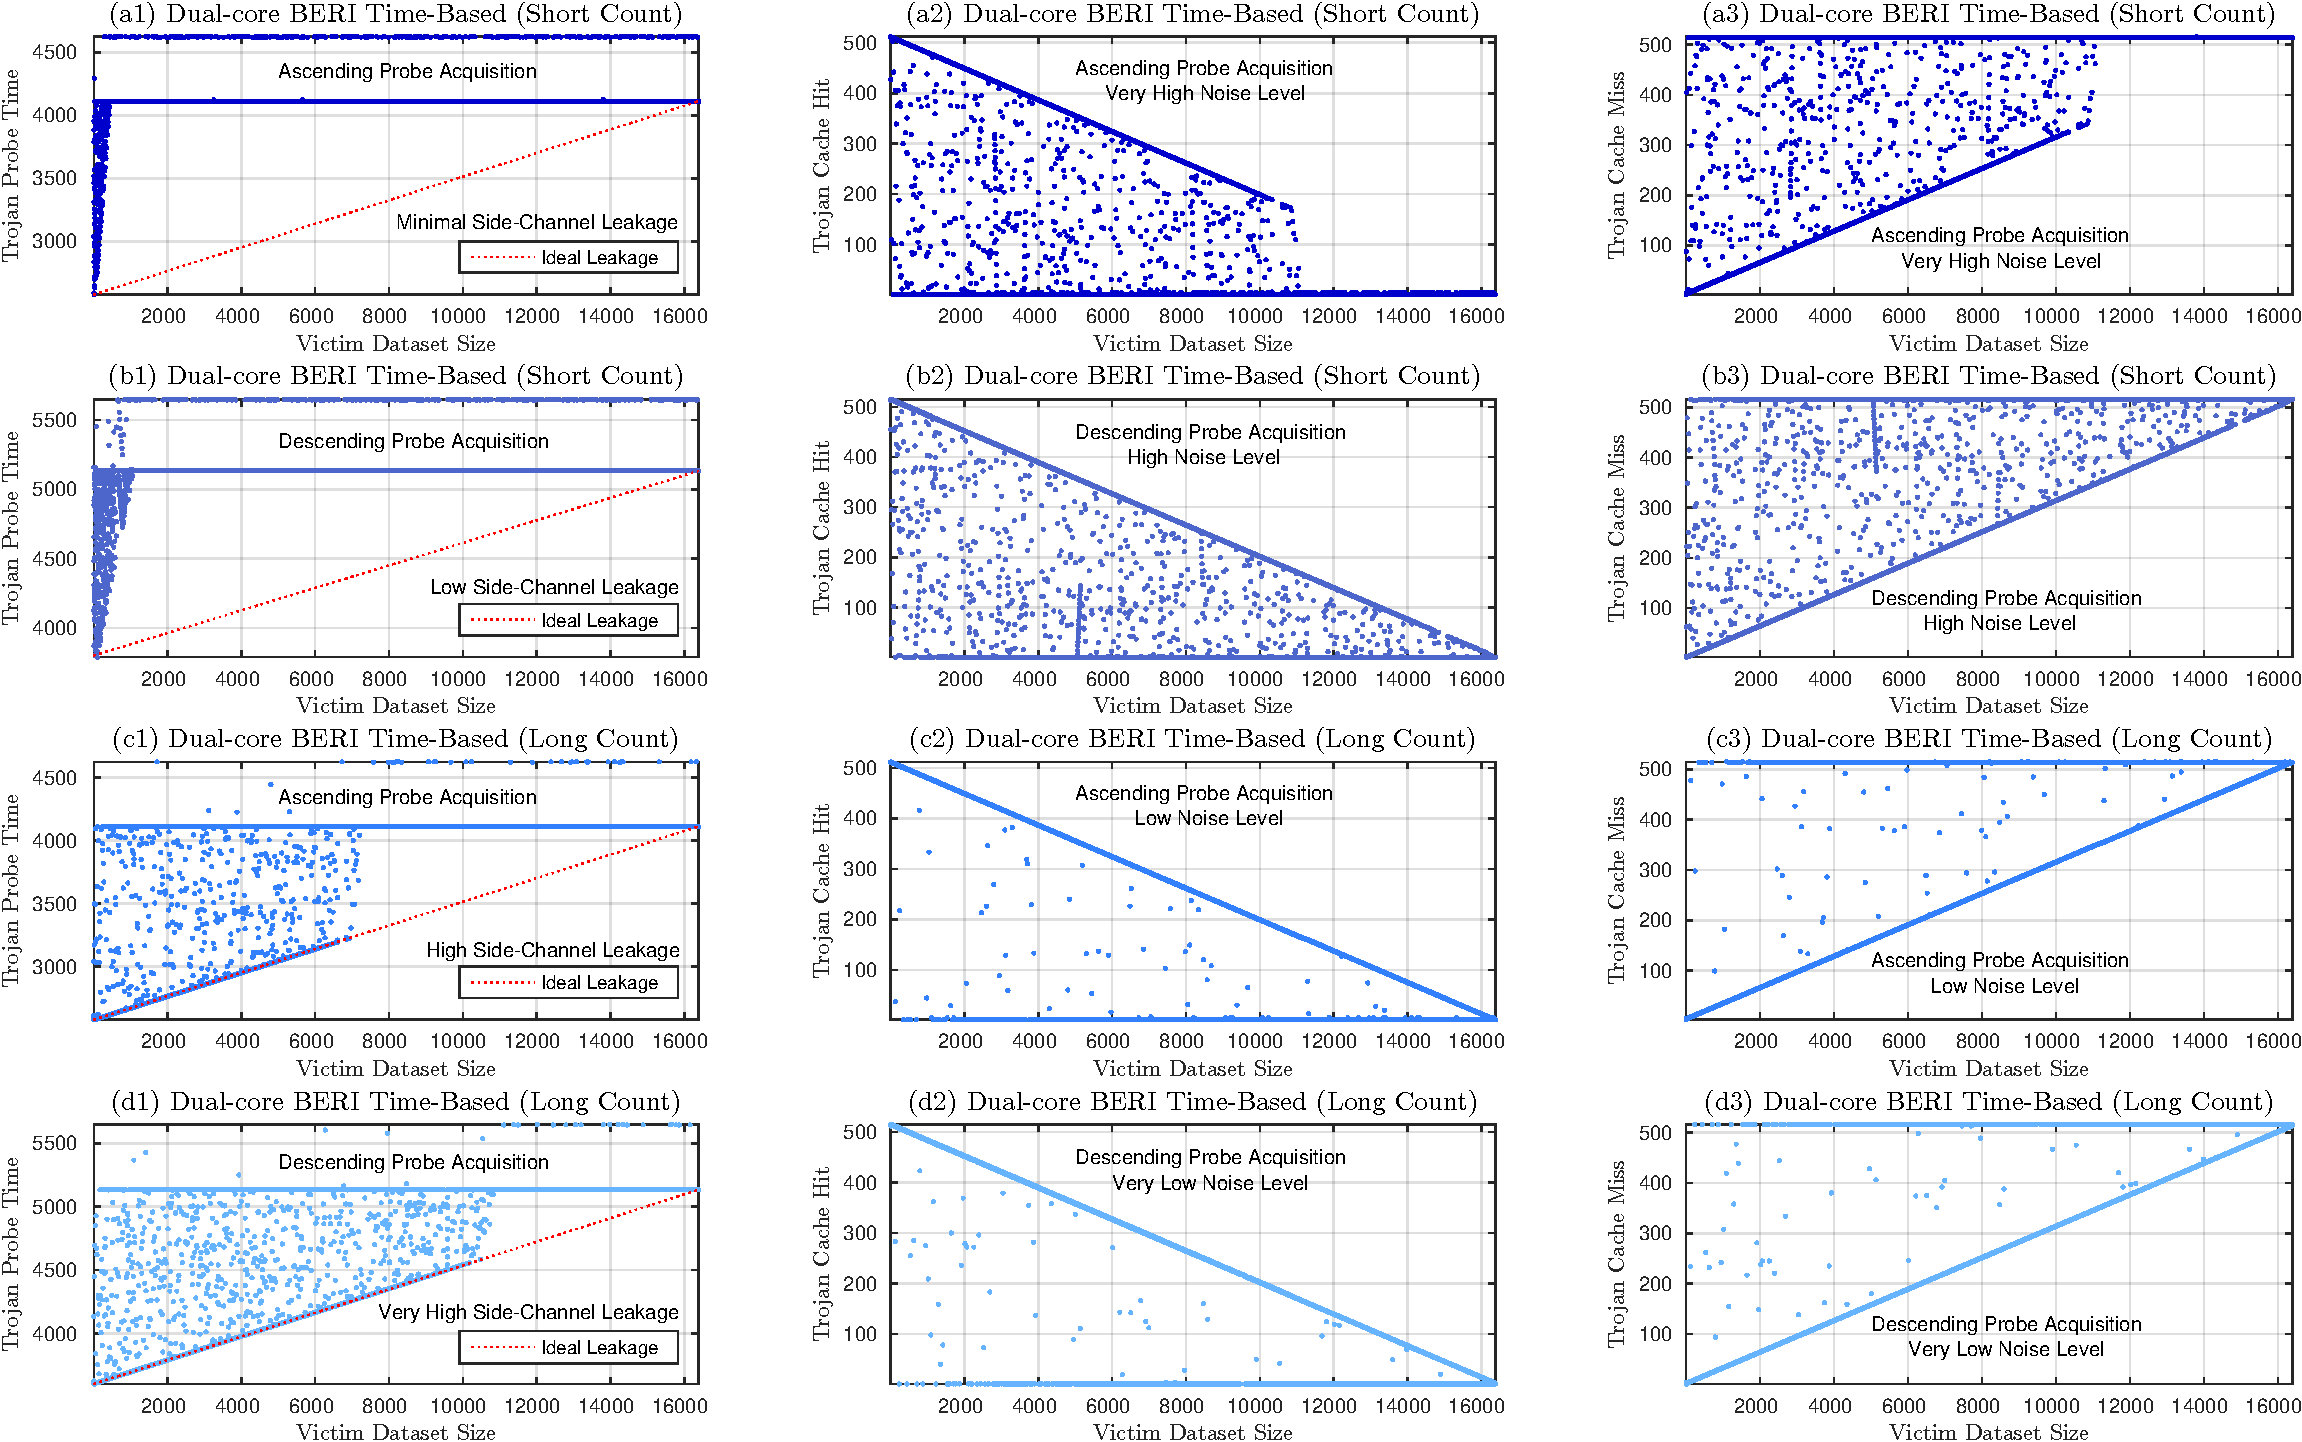
\includegraphics[width=\textheight,height=0.95\textwidth,keepaspectratio,angle=90]{sca_baremetal_reverse_1}}
						\caption{Bare metal side-channel attack, chart (3)} 
						\label{baremetal_core_pin_reverse}
					\end{figure}

\clearpage
		\subsection{Distributed Tests}
			In this test, the Trojan and Victim code segments are executed on separate cores, a highly likely scenario under OS support. The Trojan must now rely on any false sharing between its data and the Victims data in the L2 cache. The shared cache is much larger than the L1 data caches, so the likelihood of two program addresses mapping to the same cache line is lower.

			In the distributed test, Trojan code is executed on core 0 and the Victim code on core 1. Bare metal testing allows the master control program to delegate code-core allocation by reading the core ID's. During the Trojan Prime phase on core 0, core 1 is held in a wait loop. Once the Trojan completes, it signals core 1 through shared memory to begin Victim code execution. Once the Victim code completes, core 0 is signalled and the Trojan Probe phase is launched. For obvious reasons the split-core test cannot be evaluated on a single-core system.

			In order to launch the Trojan and Victim operations at the appropriate time, this test uses shared memory variables and SYNC instructions. From the description of time-based coherence so far, we have seen that stale data propagation may take a long time, to ensure quick and guaranteed updates, SYNC instructions are added after shared value updates.
			
			\paragraph{Expected Behaviour}
				The test datasets are designed to fit within the L1 data caches, so any misses will result in L2 lookups. The two cores have private L1 data caches, there will be no direct interaction between the Trojan and Victim. Memory aliasing may occur in the L2 cache which can influence the behaviour of both applications. 
				
				Time-based coherence does not provide shared memory SCA protection as it has no influence over it. In the absence of any direct memory interaction between the two codes, we do not expect to see any variation in Trojan Probe data.

			\paragraph{Observed Behaviour - Directory}
				Results match the expected behaviour, the Trojan Probe phase was not able to extract any useful information regarding the Victims dataset size. Table \ref{split_core_results} shows the obtained results. Notably the Trojan timing, miss, and hit results are constant, which is different to the time-based results.
				
				The same attack can be conducted on a larger scale, such as an L2 size Trojan Probe. Any memory aliasing between the two applications will leak exploitable side-channel information. Shared cache attacks are tested and evaluated further in this chapter.

			\paragraph{Observed Behaviour - Time-Based}
				As with the directory case, we do not observe any Trojan Probe timing fluctuations, only self-invalidation noise is present. The Trojan does encounter a higher miss rate due to self-invalidations, but the values are consistent throughout. The evaluated scheme is using a short counter offset, which has proven to provide better side-channel masking. However, this model adds performance penalties to the Victim execution, $\sim$8\%. 
				Note that the Victims execution time indirectly affects the Trojan Probe results. The wait time increases the likelihood of Trojan data self-invalidation.
				
				Two versions of the code were tested; SYNC based synchronisation and LL/SC based synchronisation. SYNC causes an immediate invalidation of all Trojan data, regardless of the Victims execution time, the Trojan always experiences maximum L1 data cache misses. The LL/SC case does not affect the time-based coherence mechanism. The Trojan may see data cache hits if the Victim execution time is low, the mean Trojan Probe cycles are slightly lower when using this synchronisation mechanism. The results show very little variation, summarised in Table \ref{split_core_results}. 
			
			\begin{table}[!h]	
			\begin{center}					
			\begin{tabular}{|l||c||c|c|}
				\hline
				\multicolumn{1}{|c||}{Parameter} & Directory & \multicolumn{2}{|c|}{Time-Based} \\
				\cline{3-4}
				& & SYNC & LL/SC \\
				\hline
				\hline
				Victim Cycles (Mean) & $\sim$77,000 & $\sim$83,000 & $\sim$83,000 \\
				Trojan Cycles & 2080 & $\sim$3650 & $\sim$3600 \\
				Probe Miss & 7 & 513 & $\sim$513 \\
				Probe Hit & 506 & 0 & $\sim$0 \\
				\hline
			\end{tabular}
			\caption{Bare metal distributed side-channel attack}
			\label{split_core_results}
			\end{center} 
			\end{table}


\clearpage
	\section{SCA Testing Including an OS}
		\label{os_prime_probe_attack}

		Performing a side-channel attack in a controlled simulation environment has precisely shown the advantages and pitfalls of using time-based coherence as a mitigation technique. Testing on an OS presents different challenges: scheduling effects, interrupts, kernel processes, and other user processes. In this set of tests the Trojan and Victim applications are the only user processes operating on the system. The bare metal code used previously was modified and recompiled to run under FreeBSD on BERI. In order to control the allocation of Victim and Trojan codes to a given core, I use the core affinity functions available for FreeBSD \cite{cpuaffinity_0,cpuaffinity_1}. 
		
		The Victim and Trojan are spawned through the same executable, however, the two applications are forked, enabling independent OS control and a different address mappings. The individual program behaviour is not modified, thus a successful attack should display results very similar to those shown in the bare metal versions. 
		
		Another significant difference in the OS tests is the timing of Trojan Probes, FreeBSD does not allow access to some hardware counters in userspace, but an OS clock function is accessible. The clock precision was sufficient to observe the expected behaviour. The hardware counter is available to use in a privileged mode but I opted out of this option since a potential attacker would not have this access.

		A total of 5 sets per test configuration were acquired, each set iteration captures 10,000 Trojan timing samples. Each timing sample is the total time taken for the Probe phase. Averaging this access time across all samples will reduce noise and provide a mean latency for a given set of test parameters. Sets are analysed individually and compared to observe any deviations. In order to improve the execution time, the bare metal test was simplified. The granularity of Victim data size increments was reduced to a total of 9 settings, starting from no data usage as a control, to full data cache capacity. 
		
		The test was also extended to Probe the L2 cache. In this version the Trojans dataset is sized to match the L2 cache. The Victim dataset is limited to the size of the L1 data cache. The Trojan Probe will incur L1 data cache misses, as the dataset is larger than L1 data cache capacity. The Probe should be able to observe misses due to evictions in the L2 cache.

		In this set of tests I use the ascending address attack. It ensures that data cache hits are not observed and all memory accesses end-up in the L2 cache, thus observing L2 cache hits and misses. 

\clearpage
		\paragraph{Figure \ref{freebsd_sca_corepin_1} --}
			This figure shows an SCA attack on the L1 data cache. The Trojan dataset size is equal to the L1 cache capacity.
			\begin{description}
			\item [(a1,b1,c1,d1)] 
				This chart group shows the median latency for the Probe phase for each Victim dataset size. Data in each chart is normalised using the minimum sample value. 
				
				The control measurement where the Victim size is zero, shows the baseline measurement. Interestingly, all the models show a consistently low value for this measurement. This is likely due to minimal interference from any other processes and other cores. 
				
				The single-core and directory versions both show a low standard deviation in values and provide the most confidence in the results. The single-core version shows a slight data deviation from the base sample to the first Victim size of 2K. This model has only one core to execute all processes, so a minimal gap between measurements will show lower interference from the rest of the system and an overall execution time. The trend line for both single-core and directory is representative of the expected behaviour and confirms the possibility of a SCA.
				
				Time-based short count version shows a high level of error and a very high miss rate for all samples other than the control. The control latency is understandable as there is no Victim execution and the Trojan Probe can begin almost immediately after the Prime phase.
				Time-counter roll-overs and L2 cache misses are also less likely in this case. 
				
				The long count model shows similar behaviour but with a much lower error rate. It still shows a flat trend for all but control samples. Some side-channel leakage is expected, as seen in the bare metal tests. 
				\textcolor{red}{The reason we may not be seeing as much leakage as the bare metal version is due to all the external factors such as the OS scheduler, interrupts and other processes.}
				Self-invalidation is very sensitive to timing so any delays inserted between the Prime and Probe phases can have profound effects on the timing results. 
			\item [(a2,b2,c2,d2)] 
				Each chart shows a normalised correlation between the acquired Probe timings and the increasing Victim memory footprint. The curves shown in charts (a1,b1,c1,d1) are compared against the Victim footprint (0K--16K \textcolor{red}{units}). 
				The single-core and directory designs, both show a strong correlation, indicating that the Trojan behaviour consistently follows the Victim behaviour. Knowing the timing curve shown in (a1,b1), we should be able to identify the memory usage of a Victim for any range that falls within the data cache.
			\end{description}

\clearpage
			\begin{figure}[!h]
			\centering 
				\makebox{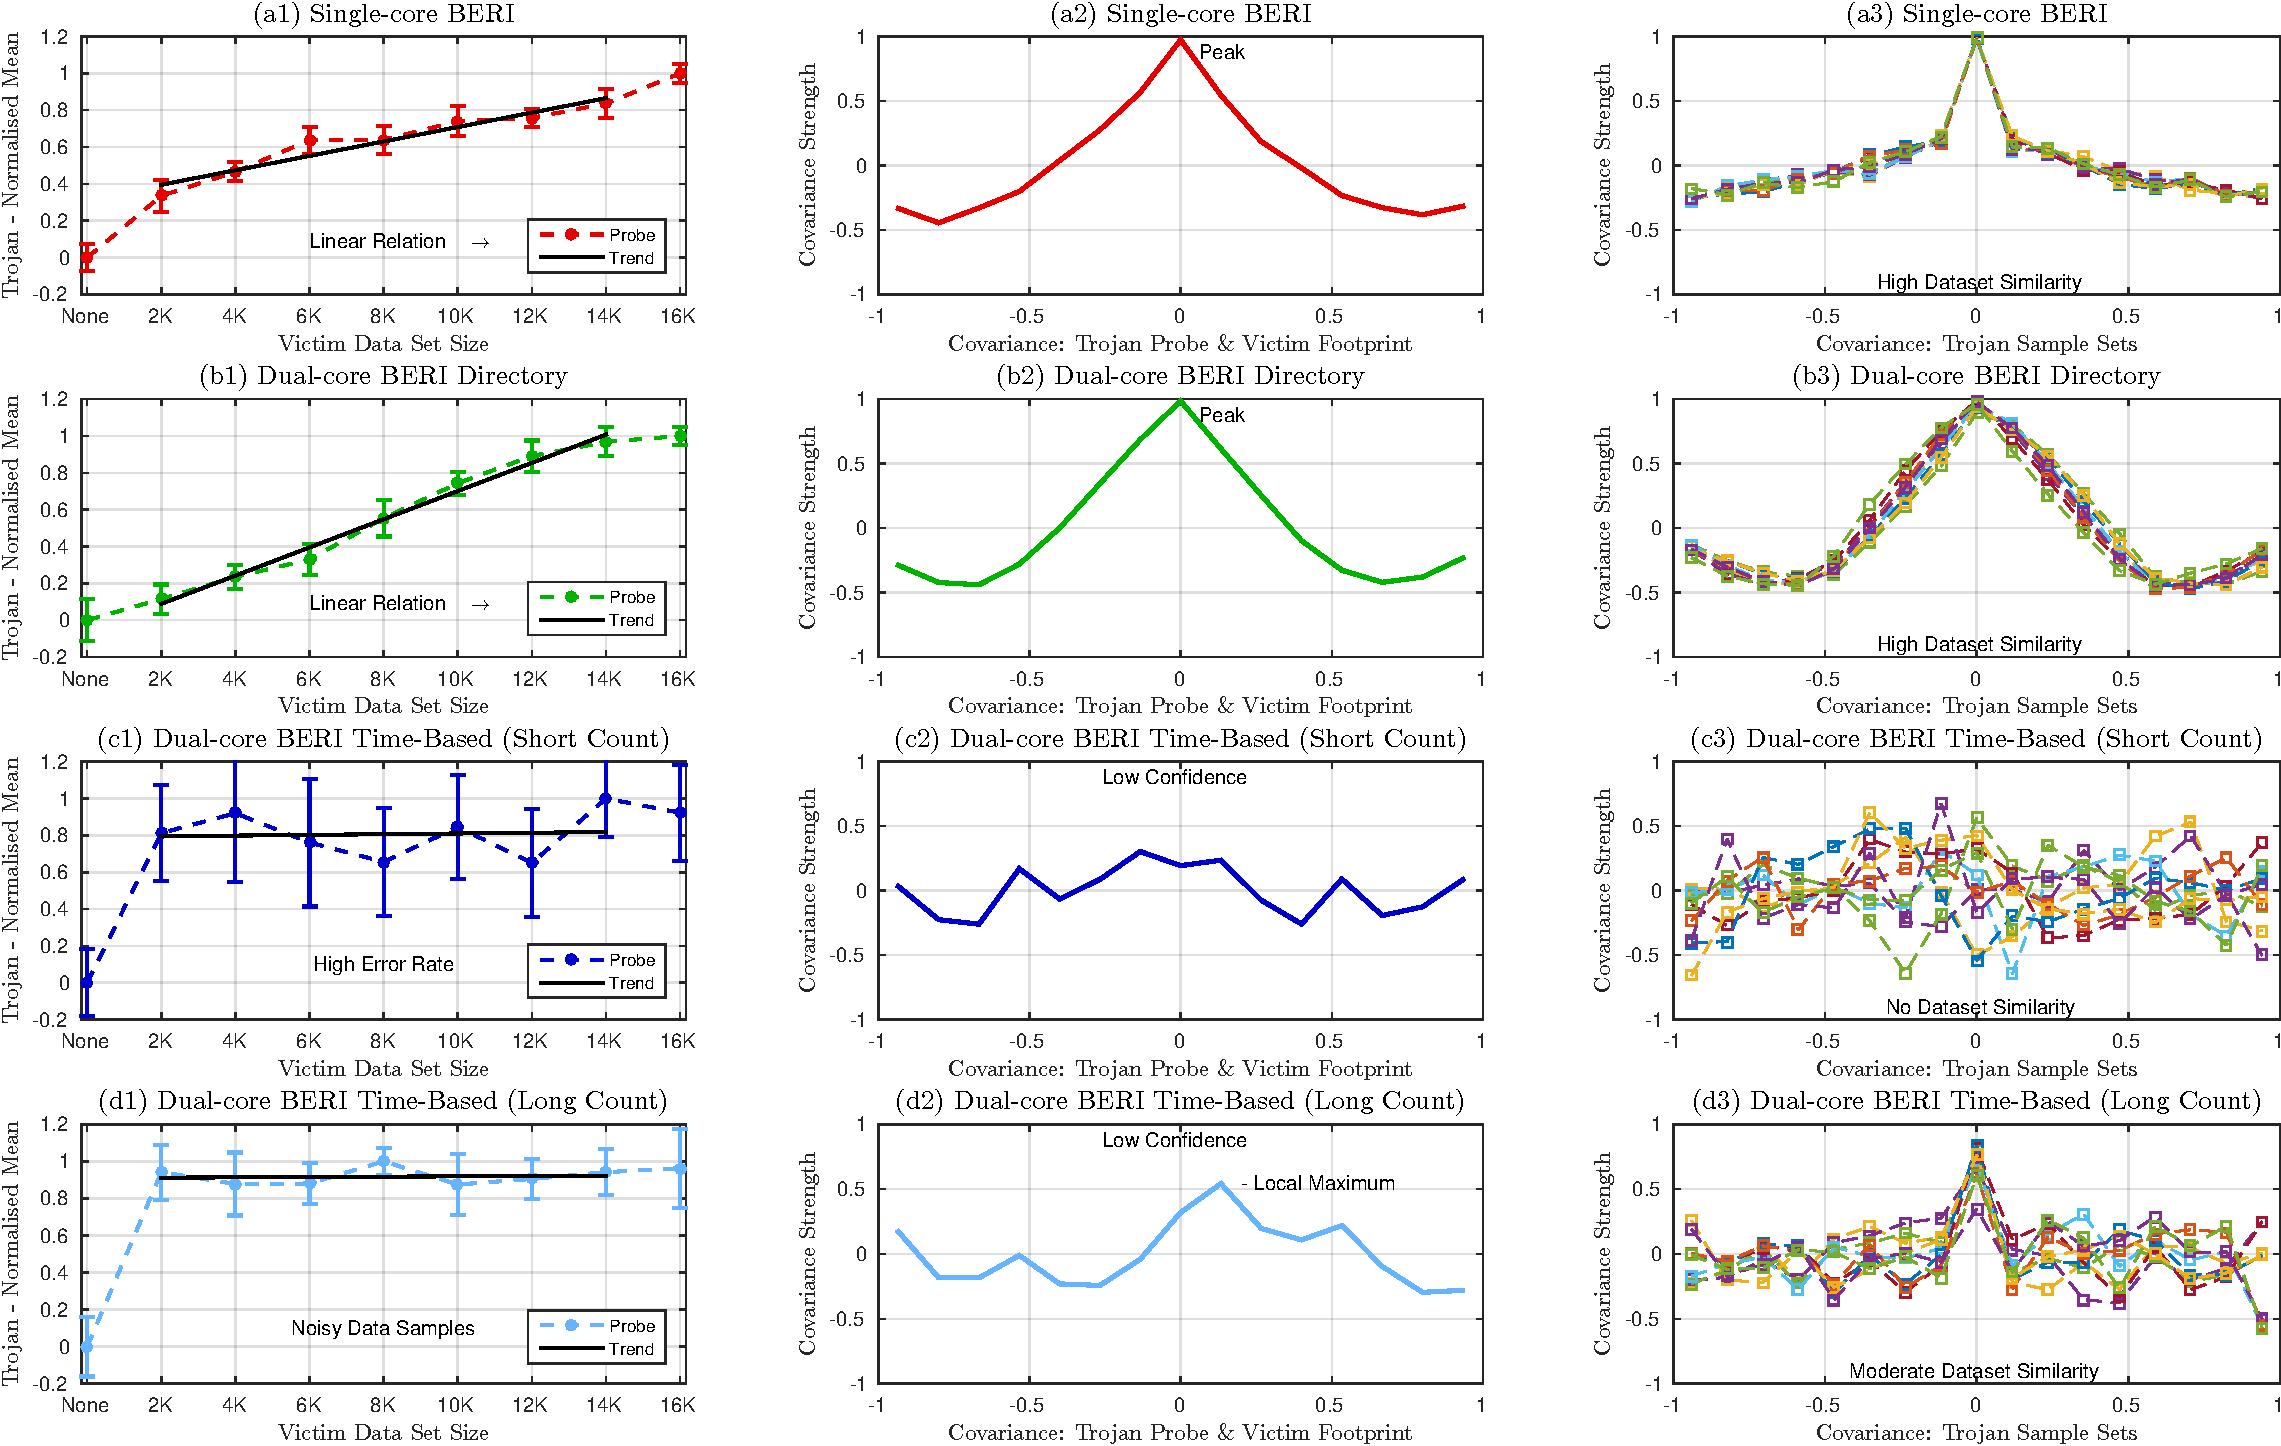
\includegraphics[width=\textheight,height=0.95\textwidth,keepaspectratio,angle=90]{freebsd_sca_corepin_1}}
				\caption{FreeBSD side-channel attack (L1 data cache)} 
				\label{freebsd_sca_corepin_1}
			\end{figure}

			\begin{figure}[!h]
			\centering 
				\makebox{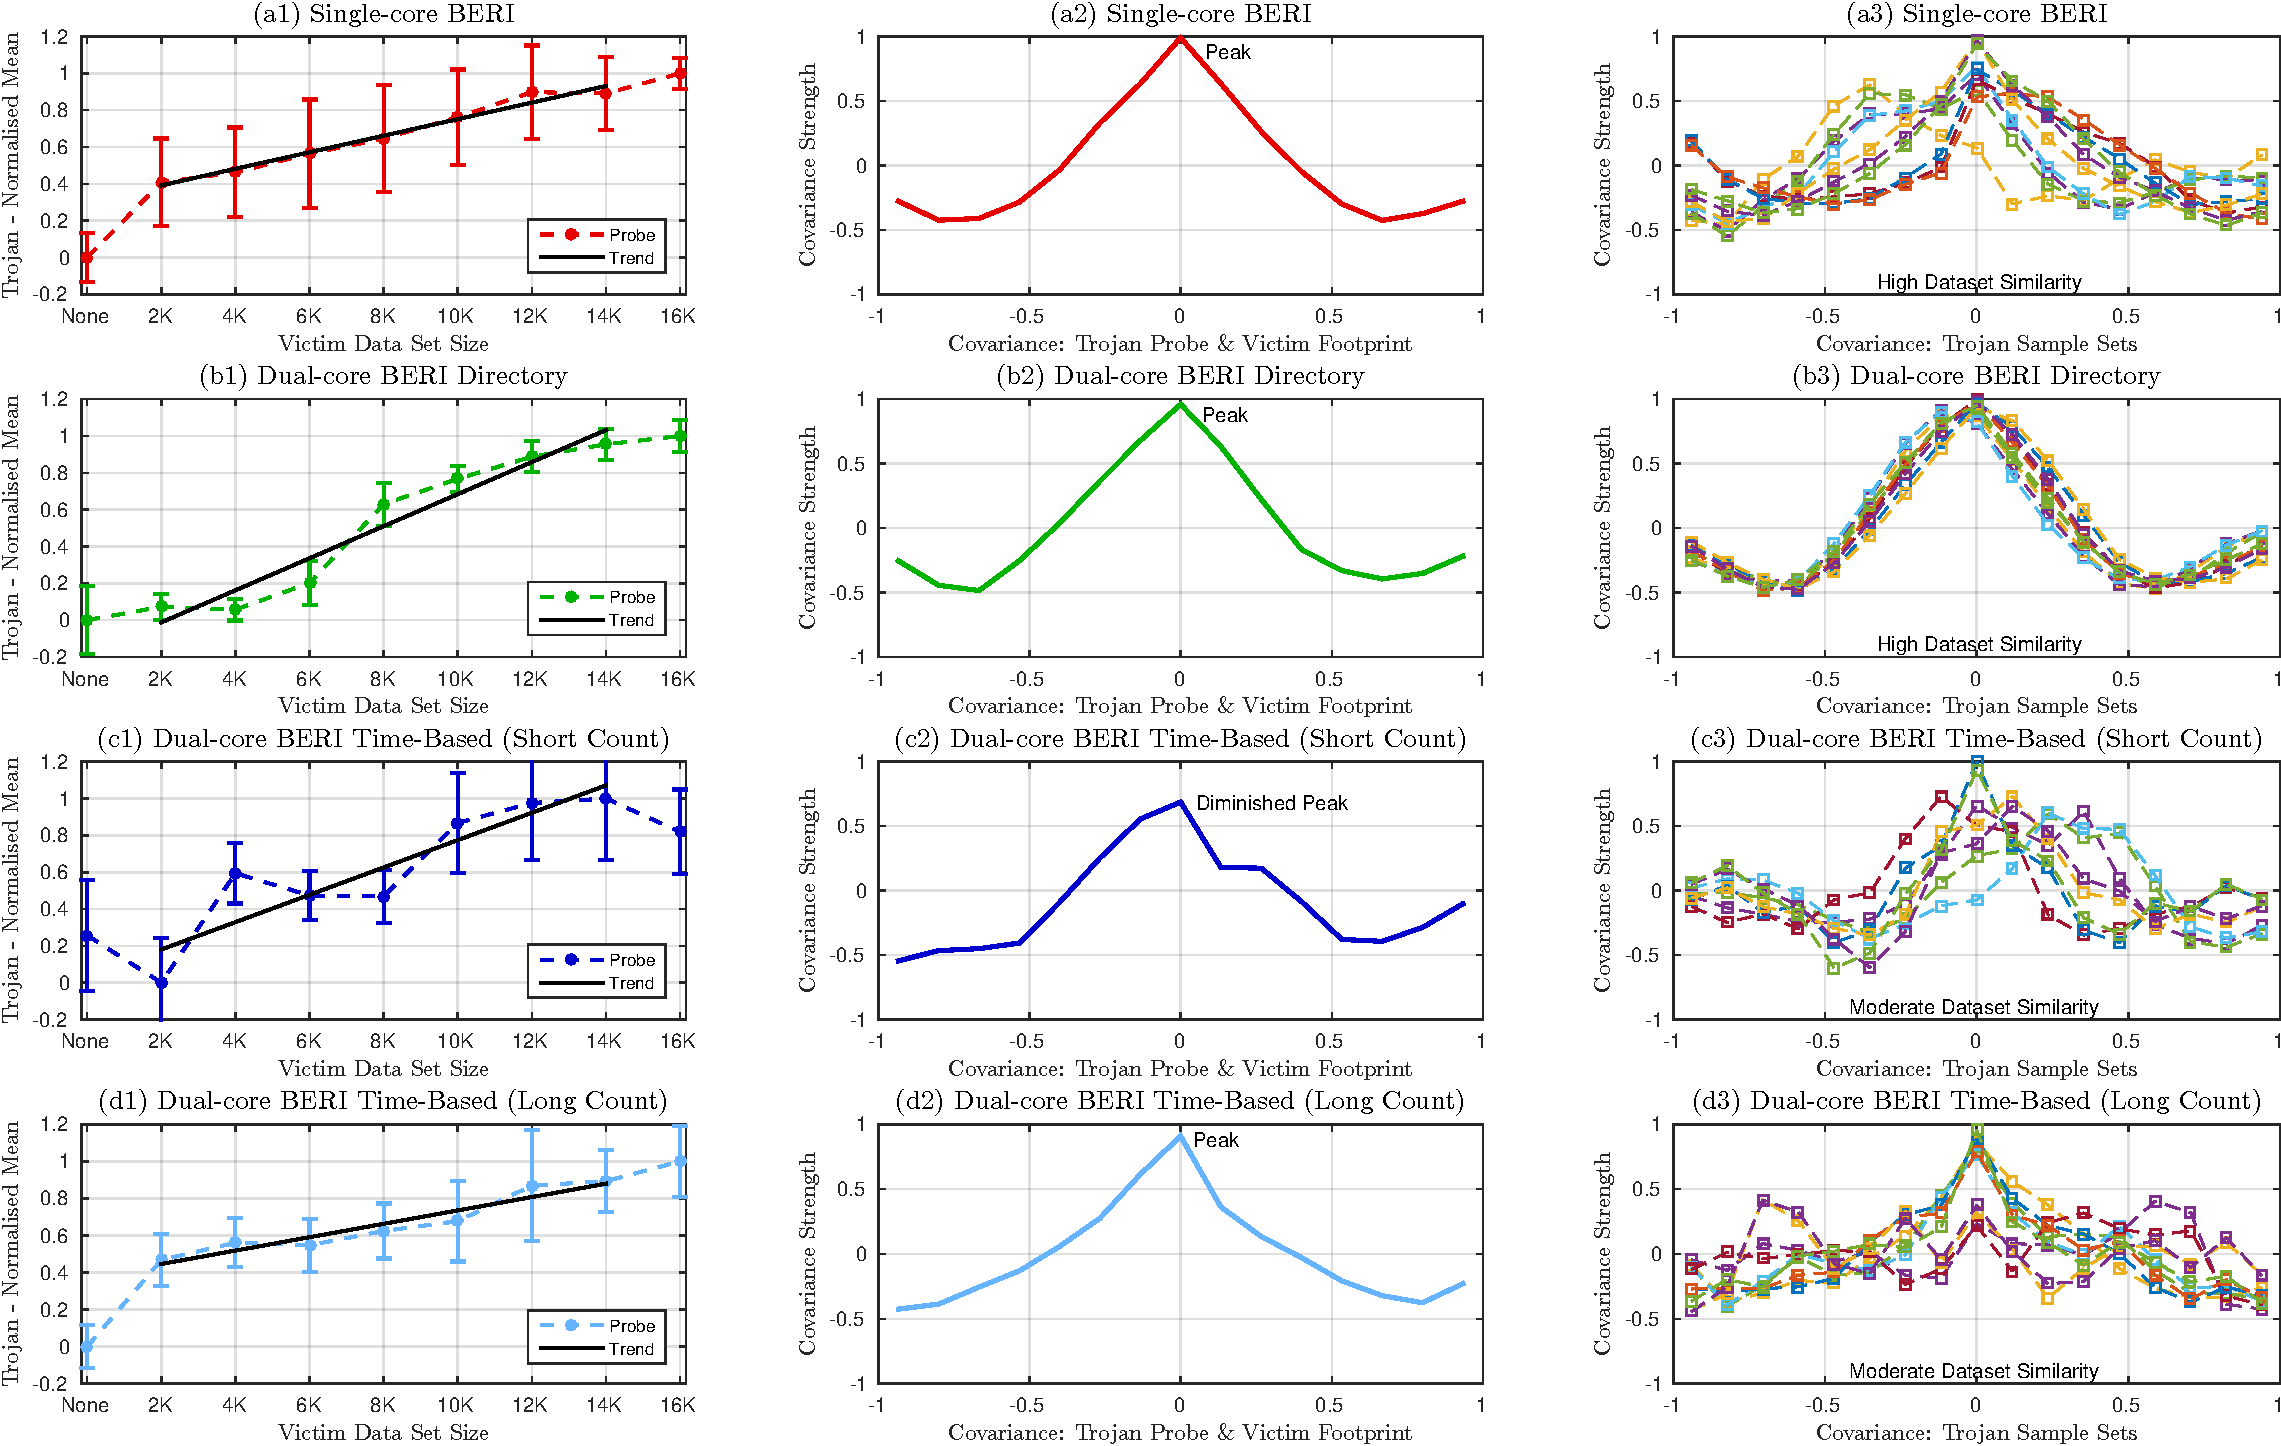
\includegraphics[width=\textheight,height=0.95\textwidth,keepaspectratio,angle=90]{freebsd_sca_corepin_2}}
				\caption{FreeBSD side-channel attack (L2 cache)} 
				\label{freebsd_sca_corepin_2}
			\end{figure}

\clearpage
			\begin{description}
			\item[\ \ \ \ \ ]
				Both time-based versions do not show a clear correlation. However, the long count version shows a minor correlation. Added Trojan sampling may be sufficient to profile this behaviour.
			\item [(a3,b3,c3,d3)] 
				In this chart we look at the similarity and reproducibility of acquired Trojan timing sets. A total of 5 sets were captured, yielding a total of 10 unique comparisons. The single-core and directory models show strong correlation between all datasets. Time-based coherence shows moderate correlation between datasets for the long count version. The short count version shows no correlation between the datasets.
			\end{description}
			
			
		\paragraph{Figure \ref{freebsd_sca_corepin_2} --}
			This figure shows an SCA attack on the L2 cache. The Trojan dataset size is equal to the L2 cache capacity.
			\begin{description}
			\item [(a1,b1,c1,d1)] 
				All charts show a common trend, Trojan time increases proportionally with an increase in the Victims dataset size. This acts as a confirmation that none of the models are protecting side-channel leakage in the shared L2 cache. Note that the observations show the mean timing information for 2048 memory accesses. The Trojan Prime phase bypasses the private cache and hits in the L2 cache. 
				
				Cache lines are not self-invalidated in the L2 so both the time-based models in (c1) and (d1) show leakage. The short count version is a little more erratic as the timing operation and general latency is likely affected by the self-invalidation mechanism. 
				
				SCAs on mechanisms such as AES require much finer timing granularity as well as the knowledge of precise latencies for each level of the cache. This test is demonstrating the amount of leakage by evaluating the average Trojan slowdown.
			\item [(a2,b2,c2,d2)] 
				The correlation charts show that each model demonstrates side-channel leakage. (c2) shows a diminished peak, however, the correlation is strong enough to profile the cache behaviour. A larger number of samples will likely present a much more accurate profile.
			\item [(a3,b3,c3,d3)] 
				The inter-set sample correlation shows that the directory provides the most reliable results out of all the models under test. Some noise is present in the single core case, likely due to other processes and interrupts. Both the time-based models are noisy, however a distinct pattern can be observed. 
			\end{description}



\clearpage
\section{Protection Level of Time-Based Coherence}
	The evaluation so far has demonstrated that time-based coherence injects some entropy into the timing data acquired by the Trojan. Several factors influence the effectiveness of this data randomisation: self-invalidation timing, critical application execution time, synchronisation instructions, the SCA target cache, number of Trojan samples, and the SCA technique.
	
	\begin{itemize}
		\item Self-Invalidation timing: The rate of data eviction in the L1 caches is directly proportional to the time-counter offset value. However, the Splash-2 benchmark results have shown that a lower time-out will cause a higher miss rate for any current application, resulting in a weaker performance. A longer time-out will improve performance but also retain the Trojan data. There is a tradeoff between application performance and side-channel leakage. Overall, time-based coherence provides more SCA mitigation than directory-based coherence, which provides none.
		%\item Application execution time: This factor ties in with self-invalidation timing, as a quicker/shorter application runtime will require a shorter self-invalidation time in order to ensure Trojan data eviction. Similarly a longer application execution time will allow using a longer TTL.
		\item Instructions: The SYNC instruction acts as a single cycle L1 data cache flush. A critical application can use this instruction before or after its execution, ensuring eviction of all L1 data. Similar techniques have been proposed and used on other systems (summarised by Osvik and Tromer \cite{Osvik06,Tromer10}), however, other systems may require explicit cache line invalidate instructions to achieve the same effect. The added instructions will cause pipeline stalls and degrade overall performance. 
		Most will argue that security overheads of the critical application are already large enough to ignore relatively small overheads caused by cache invalidate instructions, but this factor is still worth considering. One advantage of the SYNC mechanism is that the critical application requires no OS support for issuing the cache flush. Other systems may require system calls to request cache invalidation.
		\item Target cache: Time-based coherence SCA mitigation is effective in the L1 data caches. It provides no protection for the shared/last-level cache. Successful attacks on LLC's and other lower levels of memory have been demonstrated before \cite{Irazoqui15,Yarom14,Hund13,Brumley11}. Even if we can protect the LLC, attacks can be conducted on other levels of memory, such as DRAM, where other SCA techniques yield critical data. Time-based coherence can provide a level of SCA mitigation for virtual machines running on the same physical core.
		\item Trojan sampling: Time-based coherence follows a predictable self-invalidation pattern for a given cache line. A clever Trojan program may be able to carefully profile the entire cache behaviour. Repeated measurements will extract the self-invalidation timing parameters which the attacker can exploit by modifying the SCA technique. This issue can be circumvented by using software tunable dynamic self-invalidates or inserting SYNC instructions after the critical application. Even if the Trojan profiles the cache behaviour, there is little that it can do to prevent the effects of SYNC.
		\item SCA technique: In this chapter I have mostly discussed the Prime+Probe attack. It is a powerful technique when used correctly. A number of other techniques exist, these can be more or less effective against different mitigation techniques. Time-based coherence works well against Prime+Probe on L1 caches, but unlikely to defend against attacks on lower levels of memory.
	\end{itemize}
	
\section{Protecting the LLC}
\label{protecting_llc}
	The time-based coherence mechanism does not require any modifications to the LLC. We have established that the single cycle cache flush based on SYNC operations provides strong SCA protection in the private caches, a similar mechanism can be implemented in the shared cache. The LLC only needs the single cycle flush and does not require any automatic time-based self-invalidation. When the mechanism used in the private caches is integrated into the LLC, the cycle counter can be disabled. Without this counter the LLC will never perform an automatic time-based self-invalidate, thereby removing any performance drawbacks. 
		
	On SYNC instructions, the private caches can increment their local time-counters as well as propagate the instruction into the LLC. The LLC will then increment its own time-counter, thereby marking all cached data as invalid. This will guarantee side-channel masking. This scheme has some drawbacks, if the LLC is large, the resulting cache trashing will be expensive. Excessive use of SYNC instructions will cause frequent and undesirable trashing. These choices are design dependent and the need for side-channel mitigation may outweigh the drawbacks. Another drawback is that most shared caches use the write-back policy, increasing the challenge of incorporating self-invalidation, I discuss a solution to this issue in Section \ref{section_cache_properties}. Periodic flushing of dirty lines should simplify tracking lines and retain the advantages of write-back caches.

\section{Summary}
	As with many SCA mitigation techniques, time-based coherence increases the challenge of extracting useful timing information for the attacker. However, this technique is not fool proof and does not provide all aspects of SCA protection. If a system is build with this coherence model then it will possess some SCA protection out of the box, more than the standard systems. However, if any critical application is to be truly protected, other SCA mitigation techniques will be necessary. 
	
	Designers have already resorted to using dedicated hardware for both protecting and improving the performance of algorithms such as AES. Additionally, modern systems have sophisticated memory designs, allow out-of-order operations, and other optimisations, making SCAs even more challenging \cite{Tromer10,Mowery12}. Since it may not be possible to create a dedicated hardware accelerator for every critical application, software can still achieve some level of protection through our coherence model, and without a significant performance compromise.




	
% % % % % % % % % % % % % % % % % % % % % % % % % % % % % % % % % % % % % % % % % % % % % 
% % % % % % % % % % % % % % % % % % % % % % % % % % % % % % % % % % % % % % % % % % % % % 
% % % % % % % % % % % % % % % % % % % % % % % % % % % % % % % % % % % % % % % % % % % % % 
% NEW CHAPTER
% % % % % % % % % % % % % % % % % % % % % % % % % % % % % % % % % % % % % % % % % % % % % % % % % % % % % % % % % % % % % % % % % % % % % % % % % % % % % % % % % % % % % % % % % % 
% % % % % % % % % % % % % % % % % % % % % % % % % % % % % % % % % % % % % % % % % % % % % 

\chapter{Corrections: Side-Channel Attacks}
\label{chapter_sca_2}

	Some introduction here.

\section{Protection vs. Performance}
	I have already demonstrated that time-based coherence can be used to mask the side-channel leakage. However, the loss in application performance is a major drawback of this mechanism, as this technique is effective only when the cache line time-out a very frequent. This results in a poor cache usage, a higher miss rate.
	
	Another drawback of this technique is the failure to protect lower levels of memory, such as the L2 cache. Effective side-channel attacks have been demonstrated on L2 and L3 caches, DRAM's, even TLB's, and other types of memory. It is unlikely that a single mitigation technique will be effective against all attacks, for instance, a TLB level attack is likely to affect the caches and DRAM, therefore the level of protection required is very high.
	
	Side-channel masking is an inherent property of the time-based coherence protocol. This scheme can be optimised further for retaining high levels of protection, without the performance costs. And the mechanism can be extended to the L2 cache, which would allow some protection at the shared memory level.
	
	\textcolor{red}{Extend this section}
	
\section{Improved Private Cache Protection}

	Side-channel attacks designed around single threaded behaviour rely on consistent eviction of trojan data by a victim application (assuming a Prime+Probe style attack), or simply application latency based on resource contention (which also applies to multi-threaded attacks). The time-based coherence model guarantees forward progress by periodically evicting data from the private caches and also flushing the cached on barrier instructions. This property adds uncertainty to the trojan timing measurements, however, an aggressive time-based eviction policy is required to provide higher protection grantees. The drawback of an aggressive policy is the loss of performance to the victim and other applications running on the system. 
	
	A random eviction policy could improve the level of protection, but it will rely on accurate evictions of the trojan data which can not be identified by the caches. Moreover, a random eviction policy behaviour is identical or worse than an equivalent fixed delay policy. This is due to repeated measurements by the trojan application that can yield a statistically significant result. Thus, to achieve a better level of protection, the random policy is not sufficient.
	
	Cache side-channels can be avoided if the critical application forces a different cache behaviour. One such technique is ensuring a constant cache latency; hits, misses, and uncached accesses will take the same amount of time. Thus, during the execution of a critical application, all memory accesses will have a uniform timing signature but at the cost of performance. This technique will also require OS cooperation and possible hardware modifications which could include special privilege modes.
	
	The time-based model can exploit this technique by randomising memory access latency. This mechanism is orthogonal to the usual self-invalidation scheme as its triggered under certain memory access patterns. Before an application begins or ends an execution cycle, it typically performs a lock acquire or release process. The time-based scheme has been modified to observe these patterns and then randomly force cache flushes, eviction, or misses. Thus a random memory timing pattern is generated after a lock acquire/release phase. Lock typically waste machine resources (based on implementation), so the added performance penalty is negligible when evaluated with typical applications. But the side-channel protection is significantly improves over the original time-based version, while retaining the use of long cache time-outs.
	
	\textcolor{red}{Extend this section}
	
	\subsection{Attacking the Data Cache}
		This attack can be performed when the spying application runs on the same processor as the victim application. This attack can be successful when using simultaneous multi-threading or when the OS dynamically schedules processes on the same hardware thread. The attack can achieve finer granularity when the processor can execute both the spy and victim threads in parallel. The spy can constantly measure memory latency while the victim application performs some critical operations. One version of a successful attack is as following:
		
		\begin{itemize}
			\item The spy loads some data.
			\item The victim application uses the cache for its own purposes.
			\item The spy measures the time taken to reload its data. A cache hit is considered a baseline latency and the acquired time is compared to it. Based on the this time the spy can determine whether any of its data was evicted by the victim application.
		\end{itemize}
		
		If however the victim application requires more memory than the private cache capacity, the spy memory timing measurements can see if its memory was also evicted from the L2 cache. This is different to the attacks on shared memory as it can function through the local core. The spy will need to perform some profiling in order to determine the range of memory latencies.
		
		Improving SCA protection at the private cache level will also benefit from masking at shared lower memory levels. When considering only the private caches, clearing memory when switching between threads is a viable technique, but at the cost of some performance degradation. Time-based coherence will automatically clear some cache lines based on the time counters, however, SCA protection can be improved by observing typical locking patterns and then either speeding up or slowing down this flushing process.
		
		Repeated experiments can highlight the typical memory instruction patterns that are executed by critical applications can be profiled and then used to trigger SCA protection in the time-based model. In the scope of this thesis, I look at typical locking primitives such as LL/SC and use these as markers for SCA masking triggers. Locking operations are expected to be time consuming since the outcome may not always be predictable (the efficiency of these schemes varies but we can always expect some penalties). This allows the time-based model to exploit this expected performance gap and perform some cache cleaning before the next operations occur.
		
		One option would be to trigger an implicit SYNC instruction at random executions of LL/SC; we have previously established that a SYNC would flush the private caches. However, this process would be very costly due to fairly frequent occurrences of LL's and SC's. Instead, we can randomly advance the time-counter and/or force random misses on memory operations. This technique reduces the chances of a full cache flush and simply alters the memory latency of certain operations.
		
		It is important to note that when dealing with SCA's, randomising memory latency is simply an additional layer of protection. It does not guarantee full side-channel masking, instead, it makes the attack more challenging. Previous work has already demonstrated that cache locality randomisation techniques are still vulnerable to attacks, however the cache profiling method is much more demanding than with standard caches. 
	
\section{Protecting the L2}
	In the BERI multiprocessor design the L2 cache is a shared cache, used by both instruction and data caches. The time-based coherence scheme operates from within the private data caches, thus, there is no need for any coherence tracking in the shared cache. However, in order to improve the level of side-channel masking, the coherence scheme has been extended to the L2 cache. There is no need for cache line self-invalidation in the L2, but the flush on SYNC mechanism could be used to free this level of memory from any trojan data.
	
	Multiprocessor shared memory level SCAs can yield even more information than those run on single-threaded machines. Multiple applications can be executed on machines that allow simultaneous multi-threading, thus, a spy can attempt constant memory timing measurements and potentially observe the victims behaviour in real time. Therefore, any hardware security model designed to prevent shared memory attacks must be resilient to real time spying. 
	
	Caches are typically designed with features such as associativity in order to prevent core contention, false sharing, etc, etc. Associativity reduces side channel leakage when compared to a direct mapped cache. However, a cleverly designed spy application can learn the cache properties and adjust the attack model. 
	
	\subsection{Attacking Shared Memory}
		A spy application can affect memory timing by forcing its data into shared memory and then observing the latency of load operations. However, caches are typically designed to cache most frequently used data, as a result the spy data will be stored in the private cache, unless the spy application performs additional memory operations to force this data into a lower level of memory. This procedure will be more complicated if the caches are associative and designed with optimisations such as victim buffers. A general description of such an attack consists of the following steps:
		
		\begin{itemize}
			\item The spy application reads some data. On the very first occurrence, all caches and even the DRAM will incur a miss. Once the read is complete, at least one cache and the DRAM will contain a copy of this data. The presence of this data in other caches will be determined by the inclusion policy used in the system (fully inclusive on BERI).
			\item The spy reads more data in such a way that it evicts the previous copy of the data from the private cache, but doesn't evict it from the shared cache (L2). We make the following assumptions, the shared cache is larger than the private caches, and the private cache size and associativity are known or have been deduces through measurements.
			\item The spy then measures the time required to load the original piece of data. We have established that the private cache does not contain this data, but the shared cache is likely to still hold a copy. Thus, a certain latency will be observed (baseline). If any other processor or application running on the system has used shared memory to load/store some data which evicts the spy data, a higher latency will be observed.
			\item The spy can perform this set of operations repeatedly, and if required, on every cache line/word/byte in order to determine the cache usage and the granularity of measurements.
		\end{itemize}
	
		This form of an attack can be detected by a victim application as memory operations will constantly incur higher latencies. However, it will be difficult to distinguish between an attack and structural hazards.
		The attack also relies on other properties of the victim application where the program memory footprint is larger than the private cache size which will cause periodic evictions, or the victim application runs certain operations repeatedly and flushes data to the shared cache, and many other scenarios where the victim will affect the state of shared memory.
		
		In many cases the attacker is at liberty to perform repeated measurements and calculations, and the behaviour of the secure application is typically well documented and may even be open sourced. In the case of AES, the behaviour of the algorithm is well known and the spy may only need the secret key.
		
\section{Refining the Attack Model}
	It is easier to limit side-channel leakage when the spy code is executed sequentially relative to the critical application. Consequently, running the spy code in parallel with the victim allows fine grained timing measurements, and therefore higher probability of a successful attack. In order to analyse and improve the SCA protection provided by time-based coherence I have refined the attacking procedure to illustrate parallel spy execution.
	
	In the previous version of the SCA demonstrated in the initial time-based tests, the victim and trojan applications are run sequentially and after each run the timing measurements are displayed. Repeated experimentation has shown that when the attack workload is reduced (i.e. finer granularity), the measurements suffer from noise due to the print and display software calls. These calls write to a buffer using uncached writes which affect the cache behaviour for consecutive runs. In order to avoid this erroneous behaviour I have opted for measurements using the Bluespec in simulation debugging features. The display statements are independent of code execution and do not affect the cycle count of the processor. As a result, noise free fine grained measurements can be obtained. This method is somewhat representative of x86 cycle counter instructions which do no affect memory.

	Another important factor is the granularity of the critical applications operations. For instance, it is much easier to defend against an SCA when the victim accesses a cache line only once, but repeated memory accesses to this line will allow the trojan to easily observe fluctuations in memory latency to that location. The simplest way of avoiding this conflict is by using a separate mini cache for critical applications such as the ones integrated in some Intel and ARM designs. However, if the running application does not have sufficient privileges (or does not yet have a dedicated hardware unit) to use this special memory structure, it will use the regular caches which are highly susceptible to SCA's.
	
	So, how can we classify the level of protection? An ideal level of protection will eliminate any correlation between memory latency and all other applications running on the system. The spy application will observe uniform memory latency for all levels of cache. Furthermore, any attempts of the spy to push its own data to a different level of memory will be quenched by the cache. The cache will act as a completely transparent interface which is able to deliver a fixed latency memory response for all operations, regardless of complexity and side-effects. Cache designers generally strive towards this level of performance regardless of SCA masking, a transparent cache greatly simplifies the system. But such a design is difficult to achieve.
	
	In the context of BERI, a good level of protection will be offered by the caches when the memory latency signature is uniform. Whether a memory access is a hit or a miss, the response time should be identical or near identical. This can be achieved by always delaying the data cache responses, and also the L2 responses when necessary. But such a behaviour will result in CPI degradation. An improvement over this scheme would be to insert seemingly random response delays, whether an access is a hit or a miss. A performance penalty will remain, but it will lower than in the previous example.
	
\section{Spy Algorithm}
	In this description of a SCA, we will assume that the attacker has already ascertained the physical properties of the system (i.e. memory architecture, average latencies to all levels of memory, cache sizes, TLB properties, etc.). This information is vital for analysing the gathered timing information. The attack model is different for each level of memory; in this case we look at the private data caches and the shared L2 cache.
	
	\subsection{Data Cache Attack}
		In most systems the private data cache of a processor is invisible to all other processors. However, requests generated by the private caches may me visible to the rest of the memory system. Since, the private cache is invisible, an attacker must run the spy code on the same core as used by the critical application. We have already looked at Prime+Probe attacks, but in this example the granularity has been limited to a single memory location which is repeatedly timed.
		
		\paragraph{Spy's Perspective}
		\begin{enumerate}
			\item The spy application reads a memory location. On the first attempt, the data is likely to be absent from all levels of memory. However, for every repeated load, data will be returned from one of the caches unless it is evicted by other applications.
			\item The time counter instruction is executed. In this example the value is extracted through the debugging interface.
			\item The memory location is read again. 
			\item The time counter instruction is executed once again. The difference between this value and the previous time counter measurement will yield the latency of the previous memory operation.
		\end{enumerate}
	
		This procedure is susceptible to errors due to pipeline behaviour, exceptions, memory faults, etc. However, repeated measurements will display the system behaviour.
		
		\paragraph{Victim's Perspective}
			The critical application is executed as normal while the spy attempts to decipher the memory usage. The application should experience some performance loss due to memory contention. However, the fluctuations in performance will depend on the processor architecture. For instance, if the processor supports simultaneous multi-threading, the performance drop will be more noticeable. Some critical applications are designed to monitor any loss in performance and thereby detect potential side-channel attacks.
		
	\subsection{L2 Cache Attack}
		A side-channel attack at shared memory level can be conducted on separate processors, provided they are free to access and modify the same level of memory. The spy and victim codes need not be co-located. However, the spy must rely on certain properties of the victim application, such as the data set size. If the victim application uses a data set larger than the capacity of the private cache, the L2 cache will be used frequently. If the data is loaded by the application only once, the spy must detect this initial load operation. Depending on the cache behaviour, victim data writebacks could also evict the spy data which would yield side-channel information.
		
		\paragraph{Spy's Perspective}
		\begin{enumerate}
			\item The spy application reads a memory location. The spy then loads another memory location which is mapped to the same cache line as the first read. If the cache is associative, the spy may need to perform multiple loads to ensure that the first location is evicted. At this point the original location should be cached in the L2 cache, provided the subsequent memory operations did not evict that data from the L2. The main aim of this procedure is to knock out the original memory line out of the private cache.
			\item The time counter instruction is executed.
			\item Only the original memory location is read. We are not interested in the subsequent loads. This load should be a miss in the private cache but a hit in the L2. If another application has evicted the data from the L2, a miss will be observed.
			\item The time counter instruction is executed once again.
		\end{enumerate}

		\paragraph{Victim's Perspective}
			The latency observation from the victims perspective will be very different to those experienced in the private data cache side-channel attack. Sine the two applications are running on independent cores, there will be no direct interference between memory operations. If the victim application experiences private cache capacity misses, there will be a latency penalty which will be further exacerbated if the spy application causes L2 misses.

			The critical application can time the average latency of memory accesses and decide whether an attack is in process. However, shared caches are actively used by many parts of the system, and false sharing may be falsely identified as an attack. Vice versa, an active attack may be misidentified as false sharing. Thus, it is difficult to create an side-channel attack detection technique from the victims perspective. 
	
\section{Modifying Coherence Against SCA's}
	False sharing is the most common cause for side-channel leakage. This issue is further exacerbated in multiprocessor systems where the coherence management module will attempt to maintain some level of consistency throughout the system. The memory consistency model will heavily dictate side-channel leakage. For instance, a strong model such as SC or TSO will ensure that sharing information is regularly propagated through the system, but PSO or RMO relax memory orderings and do not require eager update propagation. However, weaker models will propagate many more updates on barrier operations and lead to periodic side-channel leakage. 
	
	Weaker models provide very little protection against private cache attacks, no more that strong models. But a weaker model will limit the rate of cache update propagation into shared memory, it presents a greater challenge for shared memory SCA's. The physical implementation of a strong memory consistency model will dictate the level of side-channel leakage directly due to cache coherence. Some designs limit the amount of messaging caused by false sharing, largely through a replacement policy. However, cache profiling can still detect this behaviour and thus observe the side-channels.
	
	Limiting side-channel leakage while providing reliable cache coherence and no cost to overall performance is a challenging task. A high level of SCA mitigation can be provided is the application performance is not important, not practical. This is the primary reason why manufacturers opt for dedicated hardware accelerators which largely limit SCA's while maintaining peak performance. A good example are typical cryptographic algorithms which could be use to fully encrypt a large piece of data. The timely completion of this operation may be necessary and unavoidable.
	
	\paragraph{Last level cache attacks,} particularly those relying on a cache coherence scheme are a relatively recent discovery. Only a few researchers have successfully demonstrated LLC attacks and even fewer have used the properties of cache coherence. So far the major target of attacks have been directory based protocols. 
	\begin{itemize}
		\item Cache inclusion is important, one of the reasons why attacks on AMD processors is difficult and attacks on ARM or Intel are easier. ``The LLC is a recently discovered covert channel that provides many advantages over the previous ones. First, it is a shared resource between cores, and therefore core co-residency is not needed any more. Second, LLC side channel attacks distinguish between accesses from the LLC and accesses from the memory. In contrast to the previous side channel attacks, distinguishing LLC from memory accesses can be done with a low error rate, since usually they differ in a few tens of cycles. However, these attacks have thus far only been applied to processors where the LLC is inclusive, i.e., for caches where data in the L1 cache is also present
		in the LLC.''
		\item One other advantage of AMD is a larger number of cores in their model range. As a result core collocation is difficult to achieve. However, LLC attack such as the one described in this thesis does not require core collocation.
		\item The authors of this publication use a 3 state directory protocol. The states are uncached, exclusive/modified, and shared. The protocol simpler than MESI.
		\item Some recent attacks target the memory interface itself. Modern multiprocessor systems often use proprietary interconnect hardware and protocols. However, these interfaces are designed to provide optimal performance rather than side-channel security. Two common examples are AMD's HyperTransport and Intels QuickPath Interconnect (QPI). These two interconnects are responsible for accessing different levels of memory and also to communicate coherence information. As such the attack on the memory interface is somewhat of an attack on the coherence protocol itself.
		\item Certain operating systems allow the execution of cache invalidate instructions in user space, FreeBSD does not. By executing an invalidate instruction a spy application can successfully force a data line out of shared memory, which may further trigger a coherence message to the core running the victim application. As such, when the victim accesses the data again, it will observe a miss in the private cache and then access shared memory. This access to shared memory can be visible to the spy application.
		\item Another interesting point about LLC and lower level memory attacks is the observable latency variations. It is well known that an access to every successive memory level increases the latency at an exponential rate (the exact figures vary). This of course allows the hits and misses at each level to be observed with a higher level of precision and probability. 
		\item \textcolor{red}{Note that new versions of AMD CPUs have been desinged with a non-exclusive cache inclusion policy (citation need, might be fully-inclusive). This exposes AMD CPUs to further, more advanced side-channel attacks. The main reason for this move is to improve performance, and it is clear that cache side-channel protection is not currently a priority}
	\end{itemize}
	% reference for top paragraph: https://eprint.iacr.org/2015/1155.pdf
	
	\paragraph{Attacks on ARM.} The authors of this publication list the following limitations for SCA's on ARM architectures (some of which can be overcome):
	\begin{itemize}
		\item Random cache replacement policy: This feature will result in high levels of noise in timing measurements and potentially mask all side-channel leakage.
		\item Lack of precise timing: Just like MIPS processors, on ARM the cycle count register is only available in a privileged mode. Thus, the attack assumes a rooted system, which is not required on Intel systems.
		\item Flush instructions: This is another feature reserved for privileged mode applications; unrestricted on Intel.
		\item Cache architecture: ARM did not support inclusive LLC's until the Cortex-A53/57 generation, thus presenting a similar challenge to AMD systems.
	\end{itemize}
	\begin{enumerate}
	\item The authors highlight that most modern caches use LRU eviction policies, however, they also stress that replacement policies are largely undocumented. Architects could chose a random policy over LRU as it does not require any buffering or tracking logic. 
	\item On both Linux and Windows the OS tries to minimise the memory footprint. The main focus are shared objects which are often mapped as read-only shared memory. Thus, a spy can observe any latency variations when accessing these libraries depending on the victim application demands.
	\item The ARM ISA allows different manufacturers to produce processors with some cache configuration variation. As such, the final product may have different sized L2 caches (last level cache in ARM), different inclusion levels ranging from exclusive to fully-inclusive, and other cache properties. None of these features actually prevent a SCA as the attacker may choose to run spying code on all cores and thus force a core collocated attack. `` This changed with the ARMv8-A architecture, e.g., ARM Cortex-A53 and ARM Cortex-A57 processors. On this architecture the LLC is inclusive on the instruction side and exclusive on the data side''
	\item The authors choose to attack the instruction cache. Since this private cache is inclusive the spy can simply fill the entire LLC and thus cause a miss when the instructions are loaded again (applies to all cores).
	\item Interesting fact: ``Although the data caches are exclusive, we observe that we can perform cross-core attacks on these caches as well. After evicting data from the last-level cache using memory accesses we measure higher access times. When another process running on a different core re-accesses the data we observe a lower access time again. These timing measurements would suggest an inclusive cache architecture although it is exclusive according to the documentation. We assume that this is due to the cache-coherency protocol between the CPU cores.''
	\item Performance counters are not available in user space on ARM, but newer kernels provide a unified cycle counter for all unprivileged applications. This counter access requires a syscall which adds a substantial latency overhead, however, the differences between hits and misses are still visible (Figure 3 in the paper shows this variation).
	\item ``The ARMv7-A architecture defines two different cache replacement policies, namely round-robin and pseudo-random replacement policy. In practice only the pseudo-random replacement policy is used for reasons of performance and since switching the cache replacement policy is only possible in privileged mode.'' A large dataset can overcome this issue. For highly associative caches the attacker identifies a series of congruent addresses which all map to the same cache set. Repeated accesses to these memory addresses will cause the correct cache line to be evicted consistently.
	\item The ARM ISA defines various regions of memory, sharable, exclusive, non-cachable, etc. While placing critical code into an exclusive reason gurantees no data observability from other cores, it does not mitigate cache misses due to false sharing. And placing the code into non-cachable memory does not completely alleviate the problem either, these operations can still be affected by cache usage variations, as in most cases the memory requests must pass through the cache infrastructure. And even if the caces are completely bypassed, RAM row-hammer is still a viable technique.
	\item Cache side-channel attacks are not commonly considered by major CPU manufacturers as a design priority. Thus, we can assume that this issue will become an even greater concern in the next few years. Therefore, a simple and effective solution is necessary for mitigating this security flaw. Manufacturers may be more inclined to add SCA protection as a side-effect of an existing and necessary mechanism. Of course, most manufactures such as Intel, AMD, and ARM, recommend the use of strong memory coherence and consistency models, thus a relaxed memory consistency scheme may be beyond the current scope. Note that ARM claims weak memory consistency, however, that only applies to certain memory ordering scenarious, for many shared memory operations, the ISA recommends strong ordering; the net effect is a strong memory model (further evidence found in Peter Sewells work and also the ARM ISA).
	\end{enumerate}
	% reference for top paragraph: https://online.tugraz.at/tug_online/voe_main2.getvolltext?pCurrPk=88377
	
	Let's examine four different coherence mechanisms and identify their effect on side-channel leakage (each mechanism can be tuned to produce different levels of memory consistency):
	
	\begin{table}[h]
	\begin{center}
	\begin{tabular}[c]{|l|c|c|}
		\hline
		\multicolumn{1}{|c|}{Coherence} & Consistency & Side-Channel \\
		\multicolumn{1}{|c|}{Model} & Model & Leakage \\
		\hline
		Invalidate on Write & TSO & High (baseline) \\
		BERI Directory & TSO -- RMO & High \\
		MESI Directory & TSO (likely) & Medium \\
		BERI Time-Based & RMO & Medium -- Low \\
		\hline
	\end{tabular}
	\end{center}
	\end{table}
	
	\begin{enumerate}
		\item Invalidate on Write: BERI 2016 Implementation 
		\item BERI Directory: BERI 2015 Implementation
		\item MESI Directory: No BERI Implementations 
		\item BERI Time-Based: BERI 2015 \& 2016 Implementations
	\end{enumerate}




\section{Summary}
	Cache side-channel protection is an ever growing issue and it is evident that modern CPUs do not offer many options for critical applications, let alone general applications. Furthermore, we are observing an increase in the sofhistication of SCAs, documented in academic research and proven on a variety of systems. The information regarding successful attacks on commercial systems is limitied, and potentially often undetected. 
	Is the improved LLC version of time-based coherence a viable SCA mitigation scheme? Both yes and no; it is an improvement over standard commercial systems which offer little to no protection (apart of dedicated protection for specific crypto applications), however, it does not comepltely aleviate the problem, even with the addition of protection at the LLC level.
